% ============================================================
%  template.tex —— 主文件，只写内容
%  编译方式：XeLaTeX（支持中文），编译两次生成目录
% ============================================================
\documentclass[notheorems]{beamer}

\input{pptheader.tex}
\input{mycommand.tex}

\begin{document}
	
	% ============================================================
	%  元信息：修改标题、作者、单位、日期
	% ============================================================
	\title[科研汇报]{基于高阶有限元的变密度拓扑优化}
	\subtitle{博士期间科研工作汇报}
	
	% 在 [] 中填入短作者名，避免把导师信息和排版命令也带入页脚
	\author[何亮]{报告人：何亮 \\
		\vspace{5pt}
		导师：{\CJKfontspec{SimSun}魏华祎} 教授}
	
	% [] 中填入单位简称
	\institute[湘大数学院]{
		\vspace{5pt}
		湘潭大学 \\
		数学与计算科学学院
	}
	\date{\today}
	
	% ---- 封面页 ----
	\frame[plain]{\titlepage}
	
	% ============================================================
	%  个人简介页（封面与目录之间）
	% ============================================================
	\begin{frame}[plain]
		
		\begin{tikzpicture}[remember picture, overlay]
			\fill[structure.fg]
			(current page.north west)
			rectangle ([yshift=-0.077\paperheight] current page.north east);
			\node[white, anchor=west, font=\small\bfseries\sffamily]
			at ([xshift=0.025\paperwidth, yshift=-0.038\paperheight]
			current page.north west)
			{个人简介};
			\fill[panelbg]
			([yshift=-0.077\paperheight] current page.north west)
			rectangle ([xshift=0.38\paperwidth] current page.south west);
		\end{tikzpicture}
		
		\vspace{0.077\paperheight}
		
		\begin{columns}[T, totalwidth=\linewidth]
			
			% ══════════════════════════════════════════
			% 左栏：照片 + 姓名 + 研究方向
			% ══════════════════════════════════════════
			\begin{column}{0.36\linewidth}
				\vspace{0.5em}
				\begin{center}
					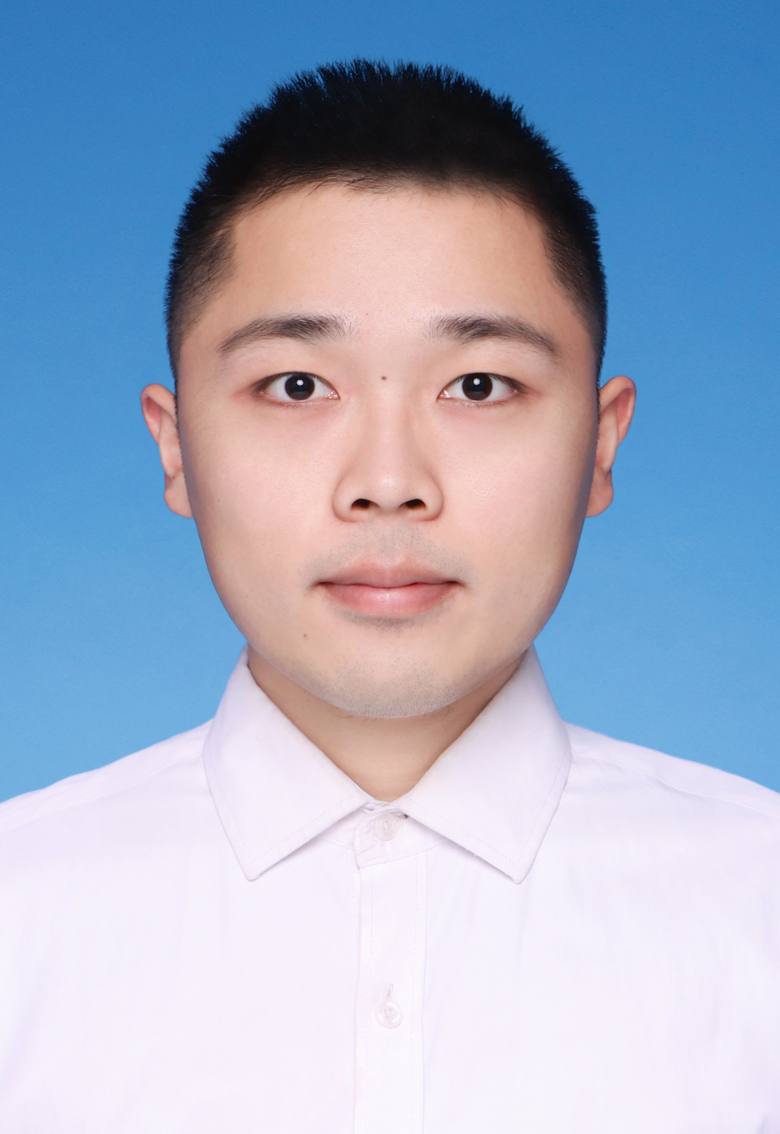
\includegraphics[width=0.50\linewidth,
					height=0.22\paperheight,
					keepaspectratio]{photo.jpg}
					
					\vspace{0.3em}
					{\fontsize{14}{18}\selectfont\bfseries\sffamily 何\quad 亮}
					
					\vspace{0.5em}
					\begin{tcolorbox}[
						colback=structure.fg, colframe=structure.fg,
						arc=4pt, boxrule=0pt,
						top=3pt, bottom=3pt, left=6pt, right=6pt,
						width=0.78\linewidth]
						\centering\color{white}\bfseries\small\sffamily 研究方向
					\end{tcolorbox}
					
					\vspace{4pt}
					% 标签：缩小字号与内边距，紧凑排列
					\tcbox[on line, arc=4pt, colback=white, colframe=tagborder,
					boxrule=0.8pt, top=1.5pt, bottom=1.5pt, left=5pt, right=5pt,
					fontupper=\footnotesize\bfseries\sffamily\color{structure.fg}]
					{偏微分方程数值方法}\\[3pt]
					\tcbox[on line, arc=4pt, colback=white, colframe=tagborder,
					boxrule=0.8pt, top=1.5pt, bottom=1.5pt, left=5pt, right=5pt,
					fontupper=\footnotesize\bfseries\sffamily\color{structure.fg}]
					{连续体结构拓扑优化}\\[3pt]
					\tcbox[on line, arc=4pt, colback=white, colframe=tagborder,
					boxrule=0.8pt, top=1.5pt, bottom=1.5pt, left=5pt, right=5pt,
					fontupper=\footnotesize\bfseries\sffamily\color{structure.fg}]
					{科学计算软件设计与实现}
				\end{center}
			\end{column}
			
			% ══════════════════════════════════════════
			% 右栏：研究主线 + 研究目标
			% ══════════════════════════════════════════
			\begin{column}{0.62\linewidth}
				\vspace{0.5em}
				
				% ── 研究主线 ────────────────────────────
				\begin{tcolorbox}[
					colback=structure.fg, colframe=structure.fg,
					arc=4pt, boxrule=0pt,
					top=3pt, bottom=3pt, left=8pt, right=8pt,
					width=\linewidth]
					\centering\color{white}\bfseries\small\sffamily 研究主线
				\end{tcolorbox}
				
				\vspace{3pt}
				{\fontsize{7.5}{10}\selectfont
					围绕基于高阶有限元的变密度拓扑优化开展系统研究，重点关注四个方面：}
				
				\vspace{4pt}
				% ── 2×2 网格 ────────────────────────────
				% 用 tabular + minipage 解决宽度与换行问题
				\begin{tabular}{@{}l@{\hspace{4pt}}l@{}}
					% 第一行
					\circnum{01}~%
					\begin{minipage}[c]{2.6cm}
						\begin{tcolorbox}[colback=panelbg!50, colframe=panelbg,
							arc=2pt, boxrule=0.5pt,
							top=2pt, bottom=2pt, left=4pt, right=4pt, nobeforeafter]
							\fontsize{7}{9}\selectfont 高阶有限元拓扑优化方法
						\end{tcolorbox}
					\end{minipage}
					&
					\circnum{03}~%
					\begin{minipage}[c]{2.6cm}
						\begin{tcolorbox}[colback=panelbg!50, colframe=panelbg,
							arc=2pt, boxrule=0.5pt,
							top=2pt, bottom=2pt, left=4pt, right=4pt, nobeforeafter]
							\fontsize{7}{9}\selectfont 胡张混合有限元拓扑优化方法
						\end{tcolorbox}
					\end{minipage}
					\\[6pt]
					% 第二行
					\circnum{02}~%
					\begin{minipage}[c]{2.6cm}
						\begin{tcolorbox}[colback=panelbg!50, colframe=panelbg,
							arc=2pt, boxrule=0.5pt,
							top=2pt, bottom=2pt, left=4pt, right=4pt, nobeforeafter]
							\fontsize{7}{9}\selectfont 多分辨率拓扑优化框架
						\end{tcolorbox}
					\end{minipage}
					&
					\circnum{04}~%
					\begin{minipage}[c]{2.6cm}
						\begin{tcolorbox}[colback=panelbg!50, colframe=panelbg,
							arc=2pt, boxrule=0.5pt,
							top=2pt, bottom=2pt, left=4pt, right=4pt, nobeforeafter]
							\fontsize{7}{9}\selectfont SOPTX 软件平台设计与实现
						\end{tcolorbox}
					\end{minipage}
				\end{tabular}
				
				\vspace{6pt}
				% ── 研究目标 ────────────────────────────
				\begin{tcolorbox}[
					colback=structure.fg, colframe=structure.fg,
					arc=4pt, boxrule=0pt,
					top=3pt, bottom=3pt, left=8pt, right=8pt,
					width=\linewidth]
					\centering\color{white}\bfseries\small\sffamily 研究目标
				\end{tcolorbox}
				
				\vspace{4pt}
				{\fontsize{8}{11}\selectfont
					面向复杂结构轻量化设计需求，围绕高精度分析、高效优化求解与软件平台实现，提升连续体结构拓扑优化的理论研究水平与工程应用能力。}
				
			\end{column}
		\end{columns}
	\end{frame}
	
	% ---- 每节开始自动插入目录页 ----
	\AtBeginSection[]{
		\frame<beamer>{
			\frametitle{目录}
			\tableofcontents[currentsection]
		}
	}
	
	% ---- 全局目录（可选） ----
	\begin{frame}
		\frametitle{目录}
		\tableofcontents
	\end{frame}
	
	
	% ============================================================
	\section{研究背景与关键问题}
	% ============================================================
	
	% ============================================================
	%  01-1  研究背景
	% ============================================================
	\begin{frame}
		\frametitle{研究背景}
		
		% ══════════════════════════════════════════════════════════
		%  中部图片区：三图横向并列，统一外框尺寸 + 居中对齐
		% ══════════════════════════════════════════════════════════
		\begin{columns}[T, totalwidth=\linewidth]
			
			\begin{column}{0.32\linewidth}
				\begin{tcolorbox}[
					enhanced, nobeforeafter,
					colback=white, colframe=structure.fg!25,
					boxrule=0.4pt, arc=2pt,
					left=3pt, right=3pt, top=4pt, bottom=4pt,
					width=\linewidth, height=0.40\paperheight,
					halign=center,
					]
					\centering
					\begin{minipage}[c][0.27\paperheight][c]{\linewidth}
						\centering
						
\includegraphics[width=\linewidth,
						height=0.27\paperheight, keepaspectratio]{aerospace}
					\end{minipage}
					\par\vspace{8pt}
					{\footnotesize\sffamily 航空航天承力结构}
				\end{tcolorbox}
			\end{column}
			
			\begin{column}{0.32\linewidth}
				\begin{tcolorbox}[
					enhanced, nobeforeafter,
					colback=white, colframe=structure.fg!25,
					boxrule=0.4pt, arc=2pt,
					left=3pt, right=3pt, top=4pt, bottom=4pt,
					width=\linewidth, height=0.40\paperheight,
					halign=center,
					]
					\centering
					\begin{minipage}[c][0.27\paperheight][c]{\linewidth}
						\centering
						
\includegraphics[width=\linewidth,
						height=0.27\paperheight, keepaspectratio]{building}
					\end{minipage}
					\par\vspace{8pt}
					{\footnotesize\sffamily 高层建筑抗侧力体系}
				\end{tcolorbox}
			\end{column}
			
			\begin{column}{0.32\linewidth}
				\begin{tcolorbox}[
					enhanced, nobeforeafter,
					colback=white, colframe=structure.fg!25,
					boxrule=0.4pt, arc=2pt,
					left=3pt, right=3pt, top=4pt, bottom=4pt,
					width=\linewidth, height=0.40\paperheight,
					halign=center,
					]
					\centering
					\begin{minipage}[c][0.27\paperheight][c]{\linewidth}
						\centering
						
\includegraphics[width=\linewidth,
						height=0.27\paperheight, keepaspectratio]{biomedical}
					\end{minipage}
					\par\vspace{8pt}
					{\footnotesize\sffamily 个性化生物医疗植入体}
				\end{tcolorbox}
			\end{column}
			
		\end{columns}
		
		\vspace{1em}
		
		% ══════════════════════════════════════════════════════════
		%  底部文字区：三条递进式结论，1/2/3 编号，左对齐
		%  采用 \makebox + \parbox 组合保证编号列与正文列精准对齐
		% ══════════════════════════════════════════════════════════
		{\fontsize{8.5}{14}\selectfont\sffamily
			\noindent
			\makebox[1.5em][l]{\textbf{1}}%
			\parbox[t]{\dimexpr\linewidth - 1.5em\relax}{%
				复杂工程结构设计对轻量化、高性能与高可靠性提出了更高要求}
			
			\vspace{5pt}\noindent
			\makebox[1.5em][l]{\textbf{2}}%
			\parbox[t]{\dimexpr\linewidth - 1.5em\relax}{%
				结构优化设计经历了由尺寸优化、形状优化到拓扑优化的递进发展}
			
			\vspace{5pt}\noindent
			\makebox[1.5em][l]{\textbf{3}}%
			\parbox[t]{\dimexpr\linewidth - 1.5em\relax}{%
				连续体结构拓扑优化以设计域内材料分布作为核心设计变量，
				是复杂结构性能驱动设计的重要数学工具}
		}
		
	\end{frame}
	
	% ============================================================
	%  01-2  关键问题
	% ============================================================
	\begin{frame}
		\frametitle{关键问题}
		
		% ── 总述条 ───────────────────────────────────────────────
		\begin{tcolorbox}[
			colback=panelbg, colframe=structure.fg!40,
			arc=3pt, boxrule=0.5pt,
			top=3pt, bottom=3pt, left=8pt, right=8pt]
			{\fontsize{8}{12}\selectfont\sffamily
				面向复杂工程应用，连续体结构拓扑优化仍面临
				高精度分析、高分辨率设计、复杂局部约束与统一软件实现等关键挑战。}
		\end{tcolorbox}
		
		\vspace{-1.2em}  % 顶部总述条与卡片之间的负间距
		
		% ── 第一行 ───────────────────────────────────────────────
		\begin{columns}[T, totalwidth=\linewidth]
			
			\begin{column}{0.485\linewidth}
				\begin{tcolorbox}[
					colback=white, colframe=structure.fg!50,
					colbacktitle=structure.fg, coltitle=white,
					fonttitle=\fontsize{8}{10}\selectfont\bfseries\sffamily,
					title={\circnum{01}\enspace 局部力学场刻画精度受限},
					arc=3pt, boxrule=0.5pt,
					toptitle=0.25pt, bottomtitle=0.25pt,
					top=3pt, bottom=3pt, left=6pt, right=6pt]
					{\fontsize{7.5}{11}\selectfont\sffamily
						\begin{itemize}
							\setlength{\itemsep}{1pt}
							\setlength{\topsep}{1pt}
							\setlength{\parsep}{0pt}
							\setlength{\parskip}{0pt}
							\item 传统低阶位移元对复杂变形与局部应力场的刻画能力有限
							\item 应力场精度不足，影响灵敏度分析与约束评估可靠性
					\end{itemize}}
				\end{tcolorbox}
			\end{column}
			
			\begin{column}{0.485\linewidth}
				\begin{tcolorbox}[
					colback=white, colframe=structure.fg!50,
					colbacktitle=structure.fg, coltitle=white,
					fonttitle=\fontsize{8}{10}\selectfont\bfseries\sffamily,
					title={\circnum{02}\enspace 分辨率与规模难以兼顾},
					arc=3pt, boxrule=0.5pt,
					toptitle=0.25pt, bottomtitle=0.25pt,
					top=3pt, bottom=3pt, left=6pt, right=6pt]
					{\fontsize{7.5}{11}\selectfont\sffamily
					\begin{itemize}
							\setlength{\itemsep}{1pt}
							\setlength{\topsep}{1pt}
							\setlength{\parsep}{0pt}
							\setlength{\parskip}{0pt}
							\item 高分辨率设计有助于获得边界清晰、细节丰富的构型
							\item 单分辨率框架下，分辨率提高通常伴随计算规模增长
					\end{itemize}}
				\end{tcolorbox}
			\end{column}
			
		\end{columns}
		
		% ── 第二行 ───────────────────────────────────────────────
		\begin{columns}[T, totalwidth=\linewidth]
			
			\begin{column}{0.485\linewidth}
				\begin{tcolorbox}[
					colback=white, colframe=structure.fg!50,
					colbacktitle=structure.fg, coltitle=white,
					fonttitle=\fontsize{8}{10}\selectfont\bfseries\sffamily,
					title={\circnum{03}\enspace 局部应力约束建模与求解困难},
					arc=3pt, boxrule=0.5pt,
					toptitle=0.25pt, bottomtitle=0.25pt,
					top=3pt, bottom=3pt, left=6pt, right=6pt]
					{\fontsize{7.5}{11}\selectfont\sffamily
					\begin{itemize}
							\setlength{\itemsep}{1pt}
							\setlength{\topsep}{1pt}
							\setlength{\parsep}{0pt}
							\setlength{\parskip}{0pt}
							\item 局部应力约束存在应力奇异性，建模与灵敏度分析困难
							\item 大量局部约束易导致优化求解困难与迭代不稳定
					\end{itemize}}
				\end{tcolorbox}
			\end{column}
			
			\begin{column}{0.485\linewidth}
				\begin{tcolorbox}[
					colback=white, colframe=structure.fg!50,
					colbacktitle=structure.fg, coltitle=white,
					fonttitle=\fontsize{8}{10}\selectfont\bfseries\sffamily,
					title={\circnum{04}\enspace 缺乏统一软件实现框架},
					arc=3pt, boxrule=0.5pt,
					toptitle=0.25pt, bottomtitle=0.25pt,
					top=3pt, bottom=3pt, left=6pt, right=6pt]
					{\fontsize{7.5}{11}\selectfont\sffamily
					\begin{itemize}
							\setlength{\itemsep}{1pt}
							\setlength{\topsep}{1pt}
							\setlength{\parsep}{0pt}
							\setlength{\parskip}{0pt}
							\item 先进数值方法与高性能计算机制缺乏统一实现框架
							\item 自动微分、多后端切换与 CPU/GPU 异构支持仍显不足
					\end{itemize}}
				\end{tcolorbox}
			\end{column}
			
		\end{columns}
		
	\end{frame}
	
	
	% ============================================================
	\section{高精度拓扑优化数值方法}
	% ============================================================
	
	% ============================================================
	%  02-1  从高阶离散到混合建模
	% ============================================================
	\begin{frame}
		\frametitle{从高阶离散到混合建模}
		
		% ── 顶部总述条 ───────────────────────────────────────────
		\begin{tcolorbox}[
			colback=panelbg, colframe=structure.fg!40,
			arc=3pt, boxrule=0.5pt,
			top=3pt, bottom=3pt, left=8pt, right=8pt]
			{\fontsize{8}{12}\selectfont\sffamily
				围绕“精度—效率—约束”三个核心问题，构建系统性高精度拓扑优化数值方法。}
		\end{tcolorbox}
		
		\vspace{-1.2em}
		
		% ══════════════════════════════════════════════════════════
		%  主体双栏：左侧关键问题 / 右侧方法路径
		% ══════════════════════════════════════════════════════════
		\begin{columns}[T, totalwidth=\linewidth]
			
			% ─── 左栏：关键科学问题 ───────────────────────────
			\begin{column}{0.485\linewidth}
				\begin{tcolorbox}[
					colback=white, colframe=structure.fg!50,
					colbacktitle=structure.fg, coltitle=white,
					fonttitle=\fontsize{8}{10}\selectfont\bfseries\sffamily,
					title={关键科学问题},
					arc=3pt, boxrule=0.5pt,
					toptitle=3pt, bottomtitle=3pt,
					top=5pt, bottom=5pt, left=6pt, right=6pt]
					{\fontsize{7.5}{11}\selectfont\sffamily
						\setbeamertemplate{enumerate item}{\fontsize{5.5}{7}\selectfont\circnum{0\insertenumlabel}}
						\begin{enumerate}
							\setlength{\itemsep}{6pt}
							\setlength{\topsep}{0pt}
							\setlength{\parsep}{0pt}
							\setlength{\parskip}{0pt}
							
							\item 局部力学场刻画精度受限，传统低阶位移元对局部应力场刻画能力有限
							
							\item 设计分辨率与规模难以兼顾，细网格带来巨大计算与存储开销
							
							\item 局部应力约束建模与求解困难，应力奇异性、局部性与大量约束并存
						\end{enumerate}
					}
				\end{tcolorbox}
			\end{column}
			
			% ─── 右栏：方法路径与技术贡献 ─────────────────────
			\begin{column}{0.485\linewidth}
				\begin{tcolorbox}[
					colback=white, colframe=structure.fg!50,
					colbacktitle=structure.fg, coltitle=white,
					fonttitle=\fontsize{8}{10}\selectfont\bfseries\sffamily,
					title={方法路径与技术贡献},
					arc=3pt, boxrule=0.5pt,
					toptitle=3pt, bottomtitle=3pt,
					top=5pt, bottom=5pt, left=6pt, right=6pt]
					{\fontsize{7.5}{11}\selectfont\sffamily
						\setbeamertemplate{enumerate item}{\fontsize{5.5}{7}\selectfont\circnum{0\insertenumlabel}}
						\begin{enumerate}
							\setlength{\itemsep}{6pt}
							\setlength{\topsep}{0pt}
							\setlength{\parsep}{0pt}
							\setlength{\parskip}{0pt}
							
							\item 任意次拉格朗日有限元方法，提升位移场及其派生应力场逼近精度
							
							\item 高阶有限元多分辨率拓扑优化框架，解耦分析网格与设计变量
							
							\item 任意次胡张混合有限元方法，直接逼近应力场，支撑局部约束可靠评估
						\end{enumerate}
					}
				\end{tcolorbox}
			\end{column}
			
		\end{columns}
		
		\vspace{0.5em}
		
		% ── 底部结论条 ───────────────────────────────────────────
		\begin{tcolorbox}[
			colback=structure.fg, colframe=structure.fg,
			arc=3pt, boxrule=0pt,
			top=4pt, bottom=4pt, left=8pt, right=8pt]
			\centering
			{\fontsize{8.5}{12}\selectfont\sffamily\color{white}
				形成\textbf{“高阶离散 — 多分辨率解耦 — 混合应力建模}"的高精度拓扑优化方法体系}
		\end{tcolorbox}
		
	\end{frame}
	
	% ============================================================
	%  02-2  任意次拉格朗日有限元拓扑优化方法
	% ============================================================
	
	\begin{frame}
		\frametitle{任意次拉格朗日有限元拓扑优化方法}
		
		% ── 顶部总述条 ───────────────────────────────────────────
		\begin{tcolorbox}[
			colback=panelbg, colframe=structure.fg!40,
			arc=3pt, boxrule=0.5pt,
			top=3pt, bottom=3pt, left=8pt, right=8pt]
			{\fontsize{8}{12}\selectfont\sffamily
				将变密度拓扑优化中的状态方程从传统低阶位移元推广到任意次拉格朗日有限元，
				构建统一的高阶离散与优化建模框架。}
		\end{tcolorbox}
		
		\vspace{-1.0em}
		
		% ── 三列卡片 ─────────────────────────────────────────────
		\begin{columns}[T, totalwidth=\linewidth]
			
			% ─── 01 高阶有限元离散 ────────────────────────────
			\begin{column}{0.325\linewidth}
				\begin{tcolorbox}[
					colback=white, colframe=structure.fg!50,
					colbacktitle=structure.fg, coltitle=white,
					fonttitle=\fontsize{8}{10}\selectfont\bfseries\sffamily,
					title={\circnum{01}\enspace 任意次有限元离散},
					arc=3pt, boxrule=0.5pt,
					toptitle=0.25pt, bottomtitle=0.25pt,
					top=3pt, bottom=3pt, left=6pt, right=6pt]
					{\fontsize{7.5}{11}\selectfont\sffamily
					\setbeamertemplate{itemize item}{\raisebox{1pt}{\tiny$\bullet$}}
					\setlength{\leftmargini}{0.85em}
						\begin{itemize}
							\setlength{\itemsep}{2pt}
							\setlength{\topsep}{1pt}
							\setlength{\parsep}{0pt}
							\setlength{\parskip}{0pt}
							\item 基于线弹性弱形式建立密度参数化状态方程
							\item 构造任意次拉格朗日有限元空间 $V_h^k$
							\item 统一支持单纯形单元与张量积单元
					\end{itemize}}
				\end{tcolorbox}
			\end{column}
			
			% ─── 02 设计变量表征 ──────────────────────────────
			\begin{column}{0.325\linewidth}
				\begin{tcolorbox}[
					colback=white, colframe=structure.fg!50,
					colbacktitle=structure.fg, coltitle=white,
					fonttitle=\fontsize{8}{10}\selectfont\bfseries\sffamily,
					title={\circnum{02}\enspace 设计变量表征},
					arc=3pt, boxrule=0.5pt,
					toptitle=0.25pt, bottomtitle=0.25pt,
					top=3pt, bottom=3pt, left=6pt, right=6pt]
					{\fontsize{7.5}{11}\selectfont\sffamily
					\setbeamertemplate{itemize item}{\raisebox{1pt}{\tiny$\bullet$}}
					\setlength{\leftmargini}{0.85em}
						\begin{itemize}
							\setlength{\itemsep}{2pt}
							\setlength{\topsep}{1pt}
							\setlength{\parsep}{0pt}
							\setlength{\parskip}{0pt}
							\item 单元密度表征：每个单元对应一个设计变量
							\item 节点密度表征：由节点变量插值构造连续密度场
							\item SIMP 材料插值：建立密度—刚度耦合关系
					\end{itemize}}
				\end{tcolorbox}
			\end{column}
			
			% ─── 03 统一比较框架 ──────────────────────────────
			\begin{column}{0.325\linewidth}
				\begin{tcolorbox}[
					colback=white, colframe=structure.fg!50,
					colbacktitle=structure.fg, coltitle=white,
					fonttitle=\fontsize{8}{10}\selectfont\bfseries\sffamily,
					title={\circnum{03}\enspace 统一比较框架},
					arc=3pt, boxrule=0.5pt,
					toptitle=0.25pt, bottomtitle=0.25pt,
					top=3pt, bottom=3pt, left=6pt, right=6pt]
					{\fontsize{7.5}{11}\selectfont\sffamily
					\setbeamertemplate{itemize item}{\raisebox{1pt}{\tiny$\bullet$}}
					\setlength{\leftmargini}{0.85em}
						\begin{itemize}
							\setlength{\itemsep}{2pt}
							\setlength{\topsep}{1pt}
							\setlength{\parsep}{0pt}
							\setlength{\parskip}{0pt}
							\item 统一载荷、边界条件、体积约束与过滤半径
							\item 比较单元类型、离散阶次与密度表征方式
							\item 评估优化构型、收敛行为与计算代价
					\end{itemize}}
				\end{tcolorbox}
			\end{column}
			
		\end{columns}
		
		\vspace{0.5em}
		
		% ── 底部总结条 ───────────────────────────────────────────
		\begin{tcolorbox}[
			colback=structure.fg, colframe=structure.fg,
			arc=3pt, boxrule=0pt,
			top=4pt, bottom=4pt, left=8pt, right=8pt]
			\centering
			{\fontsize{8.5}{12}\selectfont\sffamily\color{white}
				为系统评估高阶有限元在变密度拓扑优化中的适用性与局限性提供统一计算框架}
		\end{tcolorbox}
		
	\end{frame}
	
	% ============================================================
	%  02-3  A
	% ============================================================
	
	\begin{frame}
		\frametitle{不同离散方式与密度表征的比较}
		
		% ── 顶部总述条：随 overlay 切换 ──────────────────────────
		\begin{tcolorbox}[
			colback=panelbg, colframe=structure.fg!40,
			arc=3pt, boxrule=0.5pt,
			top=3pt, bottom=3pt, left=8pt, right=8pt]
			\only<1>{%
				\tcbox[on line, arc=3pt,
				colback=structure.fg, colframe=structure.fg,
				boxrule=0pt,
				top=1pt, bottom=1pt, left=5pt, right=5pt,
				fontupper=\fontsize{7}{9}\selectfont\bfseries\sffamily\color{white}]
				{比较维度 01：有限元离散阶次}%
				\quad
				{\fontsize{8}{12}\selectfont\sffamily
					以二维对称 MBB 梁为基准算例，在统一四边形单元、体积约束与优化参数下，比较无过滤情形中
					不同有限元阶次对优化结果的影响。}}%
			\only<2>{%
				\tcbox[on line, arc=3pt,
				colback=structure.fg, colframe=structure.fg,
				boxrule=0pt,
				top=1pt, bottom=1pt, left=5pt, right=5pt,
				fontupper=\fontsize{7}{9}\selectfont\bfseries\sffamily\color{white}]
				{比较维度 02：设计变量表征方式}%
				\quad
				{\fontsize{8}{12}\selectfont\sffamily
					在同一基准算例下，固定四边形单元、有限元阶次 $k = 2$ 与灵敏度过滤半径，
					比较单元密度与节点密度表征对优化结果的影响。}}%
			\only<3>{%
				\tcbox[on line, arc=3pt,
				colback=structure.fg, colframe=structure.fg,
				boxrule=0pt,
				top=1pt, bottom=1pt, left=5pt, right=5pt,
				fontupper=\fontsize{7}{9}\selectfont\bfseries\sffamily\color{white}]
				{比较维度 03：单元类型适用性}%
				\quad
				{\fontsize{8}{12}\selectfont\sffamily
					在同一基准算例下，固定有限元阶次 $k = 2$ 与灵敏度过滤半径，
					进一步考察三角形单元中不同密度表征方式的优化结果。}}%
		\end{tcolorbox}
		
		\vspace{-1.0em}
		
		% ── 主体内容区：overlayarea 锁高 ─────────────────────────
		\begin{overlayarea}{\linewidth}{0.50\paperheight}
			
			% ── Overlay 1：有限元离散阶次比较 ────────────────────
			\only<1>{%
				\begin{columns}[T, totalwidth=\linewidth]
					
					\begin{column}{0.325\linewidth}
						\begin{tcolorbox}[
							colback=white, colframe=structure.fg!50,
							colbacktitle=structure.fg, coltitle=white,
							fonttitle=\fontsize{8}{10}\selectfont\bfseries\sffamily,
							title={\circnum{01}\enspace 线性元 \enspace $k = 1$},
							arc=3pt, boxrule=0.5pt,
							toptitle=0.25pt, bottomtitle=0.25pt,
							top=5pt, bottom=5pt, left=5pt, right=5pt]
							\begin{center}
								
\includegraphics[width=\linewidth,
								height=0.30\paperheight, keepaspectratio]{topo_k1}
							\end{center}
							{\fontsize{7.5}{11}\selectfont\sffamily\centering\par
								$n = 53$,  $c \approx 203.07$\\
								棋盘格现象明显，边界锯齿化突出}
						\end{tcolorbox}
					\end{column}
					
					\begin{column}{0.325\linewidth}
						\begin{tcolorbox}[
							colback=white, colframe=structure.fg!50,
							colbacktitle=structure.fg, coltitle=white,
							fonttitle=\fontsize{8}{10}\selectfont\bfseries\sffamily,
							title={\circnum{02}\enspace 二阶元 \enspace $k = 2$},
							arc=3pt, boxrule=0.5pt,
							toptitle=0.25pt, bottomtitle=0.25pt,
							top=5pt, bottom=5pt, left=5pt, right=5pt]
							\begin{center}
								
\includegraphics[width=\linewidth,
								height=0.30\paperheight, keepaspectratio]{topo_k2}
							\end{center}
							{\fontsize{7.5}{11}\selectfont\sffamily\centering\par
								$n = 36$,  $c \approx 213.18$\\
								构型质量明显改善，局部伪结构减少}
						\end{tcolorbox}
					\end{column}
					
					\begin{column}{0.325\linewidth}
						\begin{tcolorbox}[
							colback=white, colframe=structure.fg!50,
							colbacktitle=structure.fg, coltitle=white,
							fonttitle=\fontsize{8}{10}\selectfont\bfseries\sffamily,
							title={\circnum{03}\enspace 四阶元 \enspace $k = 4$},
							arc=3pt, boxrule=0.5pt,
							toptitle=0.25pt, bottomtitle=0.25pt,
							top=5pt, bottom=5pt, left=5pt, right=5pt]
							\begin{center}
								
\includegraphics[width=\linewidth,
								height=0.30\paperheight, keepaspectratio]{topo_k4}
							\end{center}
							{\fontsize{7.5}{11}\selectfont\sffamily\centering\par
								$n = 41$,  $c \approx 218.66$\\
								相较 $k=2$ 改善有限，拓扑细节未同步提升}
						\end{tcolorbox}
					\end{column}
					
				\end{columns}
			}% end only<1>
			
			% ── Overlay 2：设计变量表征方式比较 ──────────────────────────
			\only<2>{%
				\begin{columns}[T, totalwidth=\linewidth]
					
					% ─── 01 单元密度表征 ─────────────────────────────
					\begin{column}{0.485\linewidth}
						\begin{tcolorbox}[
							colback=white, colframe=structure.fg!50,
							colbacktitle=structure.fg, coltitle=white,
							fonttitle=\fontsize{8}{10}\selectfont\bfseries\sffamily,
							title={\circnum{01}\enspace 单元密度表征},
							arc=3pt, boxrule=0.5pt,
							toptitle=0.25pt, bottomtitle=0.25pt,
							top=5pt, bottom=5pt, left=5pt, right=5pt,
							height=0.45\paperheight, valign=top]
							\begin{center}
								
\includegraphics[width=0.85\linewidth,
								height=0.26\paperheight, keepaspectratio]{topo_elem_density}
							\end{center}
							\vspace{-6pt}
							{\fontsize{7.5}{11}\selectfont\sffamily\centering\par
								$n = 115$,  $c \approx 226.25$\\
								宏观拓扑稳定，收敛步数较少；
								但边界阶梯化特征相对明显}
						\end{tcolorbox}
					\end{column}
					
					% ─── 02 节点密度表征 ─────────────────────────────
					\begin{column}{0.485\linewidth}
						\begin{tcolorbox}[
							colback=white, colframe=structure.fg!50,
							colbacktitle=structure.fg, coltitle=white,
							fonttitle=\fontsize{8}{10}\selectfont\bfseries\sffamily,
							title={\circnum{02}\enspace 节点密度表征},
							arc=3pt, boxrule=0.5pt,
							toptitle=0.25pt, bottomtitle=0.25pt,
							top=5pt, bottom=5pt, left=5pt, right=5pt,
							height=0.45\paperheight, valign=top]
							\begin{center}
								
\includegraphics[width=0.85\linewidth,
								height=0.30\paperheight, keepaspectratio]{topo_node_density}
							\end{center}
							\vspace{-6pt}
							{\fontsize{7.5}{11}\selectfont\sffamily\centering\par
								$n = 144$, $c \approx 229.61$\\
								宏观拓扑基本一致，边界过渡更平滑；
								但收敛步数有所增加}
						\end{tcolorbox}
					\end{column}
					
				\end{columns}
			}% end only<2>
			
			% ── Overlay 3：综合认识 ───────────────────────────────
			\only<3>{%
				\begin{columns}[T, totalwidth=\linewidth]
					
					% ─── 01 三角形单元：单元密度表 ─────────────────────────────
					\begin{column}{0.485\linewidth}
						\begin{tcolorbox}[
							colback=white, colframe=structure.fg!50,
							colbacktitle=structure.fg, coltitle=white,
							fonttitle=\fontsize{8}{10}\selectfont\bfseries\sffamily,
							title={\circnum{01}\enspace 三角形单元：单元密度表征},
							arc=3pt, boxrule=0.5pt,
							toptitle=0.25pt, bottomtitle=0.25pt,
							top=5pt, bottom=5pt, left=5pt, right=5pt,
							height=0.45\paperheight, valign=top]
							\begin{center}
								
\includegraphics[width=0.85\linewidth,
								height=0.26\paperheight, keepaspectratio]{topo_tri_elem_density}
							\end{center}
							\vspace{-6pt}
							{\fontsize{7.5}{11}\selectfont\sffamily\centering\par
								$n = 98$,  $c \approx 226.25$\\
								在三角形网格上获得稳定主承载路径，
								说明单元密度表征可自然迁移至单纯形单元。}
						\end{tcolorbox}
					\end{column}
					
					% ─── 02 三角形单元：节点密度表征 ─────────────────────────────
					\begin{column}{0.485\linewidth}
						\begin{tcolorbox}[
							colback=white, colframe=structure.fg!50,
							colbacktitle=structure.fg, coltitle=white,
							fonttitle=\fontsize{8}{10}\selectfont\bfseries\sffamily,
							title={\circnum{02}\enspace 三角形单元：节点密度表征},
							arc=3pt, boxrule=0.5pt,
							toptitle=0.25pt, bottomtitle=0.25pt,
							top=5pt, bottom=5pt, left=5pt, right=5pt,
							height=0.45\paperheight, valign=top]
							\begin{center}
								
\includegraphics[width=0.85\linewidth,
								height=0.30\paperheight, keepaspectratio]{topo_tri_node_density}
							\end{center}
							\vspace{-6pt}
							{\fontsize{7.5}{11}\selectfont\sffamily\centering\par
								$n = 109$, $c \approx 228.93$\\
								节点密度场保持连续表征优势，主拓扑特征与单元密度结果一致。}
						\end{tcolorbox}
					\end{column}
					
				\end{columns}
			}% end only<3>
			
		\end{overlayarea}
		
		% ── 底部结论条：随 overlay 切换 ──────────────────────────
		\begin{tcolorbox}[
			colback=structure.fg, colframe=structure.fg,
			arc=3pt, boxrule=0pt,
			top=4pt, bottom=4pt, left=8pt, right=8pt]
			\centering
			{\fontsize{8.5}{12}\selectfont\sffamily\color{white}
				\only<1>{提高分析阶次具有一定改善作用，但其收益受单分辨率设计空间限制}%
				\only<2>{密度表征方式影响边界过渡与收敛行为，但不能突破单分辨率框架的设计分辨率限制}%
				\only<3>{统一框架可推广至三角形单元，支撑复杂几何与非结构网格拓扑优化}
			}
		\end{tcolorbox}
		
	\end{frame}
	
	% ============================================================
	%  02-4  单分辨率框架的精度错配
	% ============================================================
	
	\begin{frame}
		\frametitle{单分辨率框架的精度错配}
		
		% ── 引导语 ───────────────────────────────────────────────
		\begin{tcolorbox}[
			colback=structure.fg!8, colframe=structure.fg!40,
			arc=2pt, boxrule=0.4pt,
			top=3pt, bottom=3pt, left=8pt, right=8pt]
			{\fontsize{8}{11}\selectfont\sffamily
				以二维对称 MBB 梁为例，考察单分辨率框架下分析精度与设计分辨率单侧提升导致的精度错配现象。}
		\end{tcolorbox}
		
		\vspace{-1.5em}
		
		% ── 主体三栏：基准 / 仅提分析精度 / 仅提设计分辨率 ───────
		\begin{columns}[T, totalwidth=\linewidth]
			
			% ─── 第一栏：基准情形 ─────────────────────────────
			\begin{column}{0.32\linewidth}
				\begin{tcolorbox}[
					colback=white, colframe=structure.fg!50,
					colbacktitle=structure.fg, coltitle=white,
					fonttitle=\fontsize{7.5}{10}\selectfont\bfseries\sffamily,
					title={\begin{minipage}[c][3.0em][c]{\linewidth}%
							\circnum{01}\enspace 基准情形:单分辨率框架，$k=2$%
					\end{minipage}},
					arc=3pt, boxrule=0.5pt,
					toptitle=0.25pt, bottomtitle=0.25pt,
					top=4pt, bottom=4pt, left=5pt, right=5pt,
					valign=top]
					\begin{center}
						
\includegraphics[width=0.92\linewidth,
						height=0.22\paperheight, keepaspectratio]{topo_baseline_k2}
					\end{center}
					{\fontsize{7}{10.5}\selectfont\sffamily\centering\par
						$\rho_{\mathrm{dof}} = 300,u_{\mathrm{dof}} = 2562$ \\[3pt]
						设计变量与分析单元绑定，限制拓扑表达分辨率}
				\end{tcolorbox}
			\end{column}
			
			% ─── 第二栏：仅提高分析精度 ───────────────────────
			\begin{column}{0.32\linewidth}
				\begin{tcolorbox}[
					colback=white, colframe=structure.fg!50,
					colbacktitle=structure.fg, coltitle=white,
					fonttitle=\fontsize{7.5}{10}\selectfont\bfseries\sffamily,
					title={\begin{minipage}[c][3.0em][c]{\linewidth}%
							\circnum{02}\enspace 仅提高分析精度：$k=2 \to 4$%
					\end{minipage}},
					arc=3pt, boxrule=0.5pt,
					toptitle=0.25pt, bottomtitle=0.25pt,
					top=4pt, bottom=4pt, left=5pt, right=5pt,
					valign=top]
					\begin{center}
						
\includegraphics[width=0.92\linewidth,
						height=0.22\paperheight, keepaspectratio]{topo_ana_k4}
					\end{center}
					{\fontsize{7}{10.5}\selectfont\sffamily\centering\par
						$\rho_{\mathrm{dof}} = 300,u_{\mathrm{dof}} = 9922\;\uparrow$ \\[3pt]
						主骨架基本一致，拓扑细节无明显改善}
				\end{tcolorbox}
			\end{column}
			
			% ─── 第三栏：仅提高设计分辨率 ─────────────────────
			\begin{column}{0.32\linewidth}
				\begin{tcolorbox}[
					colback=white, colframe=structure.fg!50,
					colbacktitle=structure.fg, coltitle=white,
					fonttitle=\fontsize{7.5}{10}\selectfont\bfseries\sffamily,
					title={\begin{minipage}[c][3.0em][c]{\linewidth}%
							\circnum{03}\enspace 仅提高设计分辨率：$4\times 4$ 子密度%
					\end{minipage}},
					arc=3pt, boxrule=0.5pt,
					toptitle=0.25pt, bottomtitle=0.25pt,
					top=4pt, bottom=4pt, left=5pt, right=5pt,
					valign=top]
					\begin{center}
						
\includegraphics[width=0.92\linewidth,
						height=0.22\paperheight, keepaspectratio]{topo_design_osc}
					\end{center}
					{\fontsize{7}{10.5}\selectfont\sffamily\centering\par
						$u_{\mathrm{dof}} = 2562,\rho_{\mathrm{dof}} = 4800\uparrow$ \\[3pt]
						出现高频震荡与局部伪结构，欠解析显著}
				\end{tcolorbox}
			\end{column}
			
		\end{columns}
		
		% ── 底部总结条 ───────────────────────────────────────────
		\begin{tcolorbox}[
			colback=structure.fg, colframe=structure.fg,
			arc=3pt, boxrule=0pt,
			top=4pt, bottom=4pt, left=8pt, right=8pt]
			\centering
			{\fontsize{8.5}{12}\selectfont\sffamily\color{white}
				设计模型与分析模型刚性绑定 $\Rightarrow$ 单侧提升难以兼顾分析精度与设计分辨率，
				需引入\textbf{多分辨率解耦机制}}
		\end{tcolorbox}
		
	\end{frame}
	
	% ============================================================
	%  02-5  高阶有限元多分辨率拓扑优化框架
	% ============================================================
	\begin{frame}
		\frametitle{高阶有限元多分辨率拓扑优化框架}
		
		% ── 引导语 ───────────────────────────────────────────────
		\begin{tcolorbox}[
			colback=structure.fg!8, colframe=structure.fg!40,
			arc=2pt, boxrule=0.4pt,
			top=3pt, bottom=3pt, left=8pt, right=8pt]
			\centering
			{\fontsize{8}{11}\selectfont\sffamily
				引入\textbf{“位移网格 — 密度积分网格 — 设计变量网格”}三层离散体系}
		\end{tcolorbox}
		
		% ── 中部：三层网格示意图（单张图） ───────────────────────
		\begin{center}
			
\includegraphics[width=0.88\linewidth, height=0.26\paperheight,
			keepaspectratio]{multires_framework}
		\end{center}
		
		\vspace{-1.5em}
		
		% ── 三栏说明 ─────────────────────────────────────────────
		\begin{columns}[T, totalwidth=\linewidth]
			
			\begin{column}{0.32\linewidth}
				\begin{tcolorbox}[
					colback=white, colframe=structure.fg!50,
					colbacktitle=structure.fg, coltitle=white,
					fonttitle=\fontsize{7.5}{10}\selectfont\bfseries\sffamily,
					title={\begin{minipage}[c][1.4em][c]{\linewidth}\centering
							$\mathcal{T}_h$\enspace 高阶位移网格
					\end{minipage}},
					arc=3pt, boxrule=0.5pt,
					toptitle=0.25pt, bottomtitle=0.25pt,
					top=4pt, bottom=4pt, left=5pt, right=5pt]
					{\fontsize{7}{10.5}\selectfont\sffamily
						采用\textbf{较粗高阶位移单元}，控制分析自由度规模}
				\end{tcolorbox}
			\end{column}
			
			\begin{column}{0.32\linewidth}
				\begin{tcolorbox}[
					colback=white, colframe=structure.fg!50,
					colbacktitle=structure.fg, coltitle=white,
					fonttitle=\fontsize{7.5}{10}\selectfont\bfseries\sffamily,
					title={\begin{minipage}[c][1.4em][c]{\linewidth}\centering
							$\mathcal{T}_\rho$\enspace 密度积分网格
					\end{minipage}},
					arc=3pt, boxrule=0.5pt,
					toptitle=0.25pt, bottomtitle=0.25pt,
					top=4pt, bottom=4pt, left=5pt, right=5pt]
					{\fontsize{7}{10.5}\selectfont\sffamily
						进行\textbf{子单元密度积分}，保证刚度组装一致性}
				\end{tcolorbox}
			\end{column}
			
			\begin{column}{0.32\linewidth}
				\begin{tcolorbox}[
					colback=white, colframe=structure.fg!50,
					colbacktitle=structure.fg, coltitle=white,
					fonttitle=\fontsize{7.5}{10}\selectfont\bfseries\sffamily,
					title={\begin{minipage}[c][1.4em][c]{\linewidth}\centering
							$\mathcal{T}_d$\enspace 设计变量网格
					\end{minipage}},
					arc=3pt, boxrule=0.5pt,
					toptitle=0.25pt, bottomtitle=0.25pt,
					top=4pt, bottom=4pt, left=5pt, right=5pt]
					{\fontsize{7}{10.5}\selectfont\sffamily
						承载\textbf{高分辨率设计变量}，提升拓扑表达能力}
				\end{tcolorbox}
			\end{column}
			
		\end{columns}
		
		\vspace{0.4em}
		
		% ── 底部结论条 ───────────────────────────────────────────
		\begin{tcolorbox}[
			colback=structure.fg, colframe=structure.fg,
			arc=3pt, boxrule=0pt,
			top=4pt, bottom=4pt, left=8pt, right=8pt]
			\centering
			{\fontsize{8.5}{12}\selectfont\sffamily\color{white}
				通过三层网格解耦，在控制计算规模的同时兼顾\textbf{高精度力学分析}与\textbf{高分辨率拓扑表达}}
		\end{tcolorbox}
		
	\end{frame}
	
	% ============================================================
	%  02-6  多分辨率框架下的拓扑表达优势
	% ============================================================
	
	\begin{frame}
		\frametitle{多分辨率框架下的拓扑表达优势}
		
		% ── 引导语 ───────────────────────────────────────────────
		\begin{tcolorbox}[
			colback=structure.fg!8, colframe=structure.fg!40,
			arc=2pt, boxrule=0.4pt,
			top=3pt, bottom=3pt, left=8pt, right=8pt]
			\centering
			{\fontsize{8}{11}\selectfont\sffamily
				以二维 MBB 梁为例，在经典密度过滤（线性映射）下展示多分辨率框架的拓扑表达优势}
		\end{tcolorbox}
		
		% ── 主体：2×2 网格（顶部标识 + 图 + 底部数据） ────────────
		\begin{center}
			\renewcommand{\arraystretch}{1.3}
			\begin{tabular}{@{}c@{\hspace{1.5em}}c@{}}
				
				% ─── (a) STOP k=1 ─────────────────────────────
				\begin{minipage}[t]{0.46\linewidth}
					\centering
					{\fontsize{8}{11}\selectfont\sffamily
						(a)\enspace STOP:\enspace $k=1,r_{\min}=1.2$\par}
					\vspace{2pt}
					
\includegraphics[width=\linewidth,
					height=0.19\paperheight, keepaspectratio]{mbb_stop_k1}\\[2pt]
					{\fontsize{7.5}{10}\selectfont\sffamily
						$\rho_{\mathrm{dof}}=600,\;u_{\mathrm{dof}}=1342$}
				\end{minipage}
				
				&
				
				% ─── (b) MTOP k=1 ─────────────────────────────
				\begin{minipage}[t]{0.46\linewidth}
					\centering
					{\fontsize{8}{11}\selectfont\sffamily
						(b)\enspace MTOP:\enspace $k=1,r_{\min}=1.0$\par}
					\vspace{2pt}
					
\includegraphics[width=\linewidth,
					height=0.19\paperheight, keepaspectratio]{mbb_mtop_k1}\\[2pt]
					{\fontsize{7.5}{10}\selectfont\sffamily
						$\rho_{\mathrm{dof}}=9600,\;u_{\mathrm{dof}}=1342$}
				\end{minipage}
				
				\\
				
				% ─── (c) MTOP k=2 ─────────────────────────────
				\begin{minipage}[t]{0.46\linewidth}
					\centering
					{\fontsize{8}{11}\selectfont\sffamily
						(c)\enspace MTOP:\enspace $k=2,r_{\min}=0.75$\par}
					\vspace{2pt}
					
\includegraphics[width=\linewidth,
					height=0.19\paperheight, keepaspectratio]{mbb_mtop_k2}\\[2pt]
					{\fontsize{7.5}{10}\selectfont\sffamily
						$\rho_{\mathrm{dof}}=9600,\;u_{\mathrm{dof}}=5082$}
				\end{minipage}
				
				&
				
				% ─── (d) MTOP k=4 ─────────────────────────────
				\begin{minipage}[t]{0.46\linewidth}
					\centering
					{\fontsize{8}{11}\selectfont\sffamily
						(d)\enspace MTOP:\enspace $k=4,r_{\min}=0.5$\par}
					\vspace{2pt}
					
\includegraphics[width=\linewidth,
					height=0.19\paperheight, keepaspectratio]{mbb_mtop_k4}\\[2pt]
					{\fontsize{7.5}{10}\selectfont\sffamily
						$\rho_{\mathrm{dof}}=9600,\;u_{\mathrm{dof}}=19762$}
				\end{minipage}
				
			\end{tabular}
		\end{center}
		
		% ── 底部结论条 ───────────────────────────────────────────
		\begin{tcolorbox}[
			colback=structure.fg, colframe=structure.fg,
			arc=3pt, boxrule=0pt,
			top=4pt, bottom=4pt, left=8pt, right=8pt]
			\centering
			{\fontsize{8.5}{12}\selectfont\sffamily\color{white}
				多分辨率解耦释放高阶有限元分析优势，获得更清晰、细节更丰富的拓扑构型}
		\end{tcolorbox}
		
	\end{frame}
	
	% ============================================================
	%  02-7  密度映射机制与构型鲁棒性
	% ============================================================
	
	\begin{frame}
		\frametitle{密度映射机制与构型鲁棒性}
		
		% ── 引导语 ───────────────────────────────────────────────
		\begin{tcolorbox}[
			colback=structure.fg!8, colframe=structure.fg!40,
			arc=2pt, boxrule=0.4pt,
			top=3pt, bottom=3pt, left=8pt, right=8pt]
			\centering
			{\fontsize{8}{11}\selectfont\sffamily
				在三层多分辨率框架下，进一步比较不同密度映射机制对拓扑构型与算法稳定性的影响}
		\end{tcolorbox}
		
		% ── 左右两栏对照 ──────────────────────────────────────────
		\begin{columns}[T, totalwidth=\linewidth]
			
			% ─── 左栏：灵敏度过滤（恒等映射）─────────────────
			\begin{column}{0.485\linewidth}
				\centering
				% 栏目标题 
				{\fontsize{9}{10}\selectfont\sffamily\bfseries\color{structure.fg}
					灵敏度过滤：恒等映射\par}
					
				\vspace{2pt}
				
				% 子图 1：k=1
				
\includegraphics[width=0.92\linewidth, height=0.18\paperheight,
				keepaspectratio]{filter_identity_k1}\\[1pt]
				{\fontsize{7.5}{10}\selectfont\sffamily (a)\enspace $k=1,r_{\min}=1.0$}
				
				\vspace{4pt}
				
				% 子图 2：k=4
				
\includegraphics[width=0.92\linewidth, height=0.18\paperheight,
				keepaspectratio]{filter_identity_k4}\\[1pt]
				{\fontsize{7.5}{10}\selectfont\sffamily (b)\enspace $k=4,r_{\min}=0.5$}
				
				\vspace{6pt}
				% 说明
				{\fontsize{7.5}{11}\selectfont\sffamily
					设计变量与物理密度直接对应，构型演化较稳定，但边界灰度过渡较明显}
			\end{column}
			
			% ─── 右栏：非线性投影（复合映射）─────────────────
			\begin{column}{0.485\linewidth}
				\centering
				% 栏目标题 
				{\fontsize{9}{10}\selectfont\sffamily\bfseries\color{structure.fg}
					非线性投影：复合映射\par}
					
				\vspace{2pt}
				
				% 子图 1：k=1
				
\includegraphics[width=0.92\linewidth, height=0.18\paperheight,
				keepaspectratio]{projection_composite_k1}\\[1pt]
				{\fontsize{7.5}{10}\selectfont\sffamily (c)\enspace $k=1,r_{\min}=1.0$}
				
				\vspace{4pt}
				
				% 子图 2：k=4
				
\includegraphics[width=0.92\linewidth, height=0.18\paperheight,
				keepaspectratio]{projection_composite_k4}\\[1pt]
				{\fontsize{7.5}{10}\selectfont\sffamily (d)\enspace $k=4,r_{\min}=0.5$}
				
				\vspace{6pt}
				% 说明
				{\fontsize{7.5}{11}\selectfont\sffamily
					投影增强 0–1 二值化特征，高阶分析下边界更清晰、细节更丰富}
			\end{column}
			
		\end{columns}
		
		% ── 底部结论条 ───────────────────────────────────────────
		\begin{tcolorbox}[
			colback=structure.fg, colframe=structure.fg,
			arc=3pt, boxrule=0pt,
			top=4pt, bottom=4pt, left=8pt, right=8pt]
			\centering
			{\fontsize{8.5}{12}\selectfont\sffamily\color{white}
				将过滤、投影与高阶分析协同耦合，提升了多分辨率拓扑优化的构型质量与算法鲁棒性}
		\end{tcolorbox}
		
	\end{frame}
	
	% ============================================================
	%  02-8  多分辨率框架在应力约束问题中的应用
	% ============================================================
	
	\begin{frame}
		\frametitle{多分辨率框架在应力约束问题中的应用}
		
		% ── 引导语 ───────────────────────────────────────────────
		\begin{tcolorbox}[
			colback=structure.fg!8, colframe=structure.fg!40,
			arc=2pt, boxrule=0.4pt,
			top=3pt, bottom=3pt, left=8pt, right=8pt]
			\centering
			{\fontsize{8}{11}\selectfont\sffamily
				以 L 型支架为例，在多分辨率框架下考察高阶有限元分析对应力约束拓扑结果的影响}
		\end{tcolorbox}
		
%		\vspace{0.5em}
		
		% ── 双主列嵌套布局 ───────────────────────────────────────
		\begin{columns}[T, totalwidth=\linewidth]
			
			% ════════════ 左主列：最终优化拓扑构型 ════════════
			\begin{column}{0.48\linewidth}\centering
				{\fontsize{9}{11}\selectfont\sffamily\bfseries\color{structure.fg}
					最终优化拓扑构型\par}
				
				% 嵌套子列：并排展示 k=1 和 k=4
				\begin{columns}[T, totalwidth=\linewidth]
					\begin{column}{0.48\linewidth}\centering
						
\includegraphics[width=\linewidth, keepaspectratio]{lbracket_topo_k1}\vspace{2pt}
						{\fontsize{8}{10}\selectfont\sffamily $k=1,r_{\min}=1.0$\par}
					\end{column}
					\begin{column}{0.48\linewidth}\centering
						
\includegraphics[width=\linewidth, keepaspectratio]{lbracket_topo_k4}\vspace{2pt}
						{\fontsize{8}{10}\selectfont\sffamily $k=4,r_{\min}=0.5$\par}
					\end{column}
				\end{columns}
			\end{column}
			
			% 中间间距
			\begin{column}{0.02\linewidth}\end{column}
			
			% ════════════ 右主列：归一化 von Mises 等效应力 ════════════
			\begin{column}{0.48\linewidth}\centering
				{\fontsize{9}{11}\selectfont\sffamily\bfseries\color{structure.fg}
					归一化 von Mises 等效应力\par}
				
				% 嵌套子列：并排展示 k=1 和 k=4
				\begin{columns}[T, totalwidth=\linewidth]
					\begin{column}{0.48\linewidth}\centering
						
\includegraphics[width=\linewidth, keepaspectratio]{lbracket_stress_k1}\vspace{2pt}
						{\fontsize{8}{10}\selectfont\sffamily $k=1,r_{\min}=1.0$\par}
					\end{column}
					\begin{column}{0.48\linewidth}\centering
						
\includegraphics[width=\linewidth, keepaspectratio]{lbracket_stress_k4}\vspace{2pt}
						{\fontsize{8}{10}\selectfont\sffamily $k=4,r_{\min}=0.5$\par}
					\end{column}
				\end{columns}
			\end{column}
			
		\end{columns}
		
		\vspace{1em}
		
		% ── 底部结论条 ───────────────────────────────────────────
		\begin{tcolorbox}[
			colback=structure.fg, colframe=structure.fg,
			arc=3pt, boxrule=0pt,
			top=4pt, bottom=4pt, left=8pt, right=8pt]
			\centering
			{\fontsize{8.5}{12}\selectfont\sffamily\color{white}
				多分辨率框架可用于 L 型支架局部应力约束优化；
				进一步提升应力场逼近质量，需要引入混合有限元方法}
		\end{tcolorbox}
		
	\end{frame}
	
	% ============================================================
	%  02-9  从位移法到混合应力建模
	% ============================================================
	
	\begin{frame}
		\frametitle{从位移法到混合应力建模}
		
		% ── 引导语 ───────────────────────────────────────────────
		\begin{tcolorbox}[
			colback=structure.fg!8, colframe=structure.fg!40,
			arc=2pt, boxrule=0.4pt,
			top=3pt, bottom=3pt, left=8pt, right=8pt]
			{\fontsize{8}{11}\selectfont\sffamily
				前述高阶有限元与多分辨率框架提升了位移场分析精度与拓扑表达能力；
				面向近不可压缩材料和局部应力约束，仍需更可靠的应力场建模方法。}
		\end{tcolorbox}
		
		\vspace{-1.5em}
		
		% ── 主体双栏：局限性 vs 解决思路 ───────────────────────────
		\begin{columns}[T, totalwidth=\linewidth]
			
			% ════════ 左栏：位移型有限元的局限 ════════
			\begin{column}{0.485\linewidth}
				\begin{tcolorbox}[
					colback=white, colframe=structure.fg!50,
					colbacktitle=structure.fg, coltitle=white,
					fonttitle=\fontsize{8}{10}\selectfont\bfseries\sffamily,
					title={位移型有限元的局限},
					arc=3pt, boxrule=0.5pt,
					toptitle=3pt, bottomtitle=3pt,
					top=5pt, bottom=5pt, left=6pt, right=6pt,
					height=0.45\paperheight, valign=top] % 锁高保证左右对齐
					{\fontsize{7.5}{11}\selectfont\sffamily
						
						\textbf{\circnum{01}\enspace 近不可压缩材料}\par
						\vspace{2pt}
						泊松比 $\nu \to 0.5$ 时，位移型有限元易出现体积闭锁，导致刚度高估与非物理拓扑演化。
						
						\vspace{8pt}
						\textbf{\circnum{02}\enspace 局部应力场评估}\par
						\vspace{2pt}
						应力由位移梯度派生得到，跨单元通常不连续，局部应力集中与约束评估精度受限。
					}
				\end{tcolorbox}
			\end{column}
			
			% ════════ 右栏：混合应力建模思路 ════════
			\begin{column}{0.485\linewidth}
				\begin{tcolorbox}[
					colback=white, colframe=structure.fg!50,
					colbacktitle=structure.fg, coltitle=white,
					fonttitle=\fontsize{8}{10}\selectfont\bfseries\sffamily,
					title={混合应力建模思路},
					arc=3pt, boxrule=0.5pt,
					toptitle=3pt, bottomtitle=3pt,
					top=5pt, bottom=5pt, left=6pt, right=6pt,
					height=0.45\paperheight, valign=top] % 锁高保证左右对齐
					{\fontsize{7.5}{11}\selectfont\sffamily

						\textbf{\circnum{01}\enspace 应力—位移混合建模}\par
						\vspace{2pt}
						基于 Hellinger–Reissner 原理，将应力 $\boldsymbol{\sigma}$ 与位移 $\boldsymbol{u}$ 同时作为未知量求解，提高应力精度。
						
						\vspace{8pt}
						\textbf{\circnum{02}\enspace 面向复杂局部约束}\par
						\vspace{2pt}
						构造 $H(\text{div})$ 协调应力空间，为近不可压缩与局部应力约束评估提供稳定支撑。
					}
				\end{tcolorbox}
			\end{column}
			
		\end{columns}
		
		% ── 底部结论条 ───────────────────────────────────────────
		\begin{tcolorbox}[
			colback=structure.fg, colframe=structure.fg,
			arc=3pt, boxrule=0pt,
			top=4pt, bottom=4pt, left=8pt, right=8pt]
			\centering
			{\fontsize{8.5}{12}\selectfont\sffamily\color{white}
				从“位移导出应力”转向“应力—位移混合求解”，推动拓扑优化从位移场高精度分析进一步走向应力场高精度建模。}
		\end{tcolorbox}
		
	\end{frame}
	
	% ============================================================
	%  02-10  任意次胡张混合有限元
	% ============================================================
	
	\begin{frame}
		\frametitle{任意次胡张混合有限元方法}
		
		% ── 引导语 ───────────────────────────────────────────────
		\begin{tcolorbox}[
			colback=structure.fg!8, colframe=structure.fg!40,
			arc=2pt, boxrule=0.4pt,
			top=3pt, bottom=3pt, left=8pt, right=8pt]
			{\fontsize{8}{11}\selectfont\sffamily
				基于北京大学胡俊教授提出并发展的任意次单纯形胡张混合有限元，
				完成程序实现，并系统引入变密度拓扑优化框架。}
		\end{tcolorbox}
		
		\vspace{-1.5em}
		
		% ── 主体双栏：离散实现 vs 优化闭环 ───────────────────────────
		\begin{columns}[T, totalwidth=\linewidth]
			
			% ════════ 左栏：任意次胡张元实现 ════════
			\begin{column}{0.485\linewidth}
				\begin{tcolorbox}[
					colback=white, colframe=structure.fg!50,
					colbacktitle=structure.fg, coltitle=white,
					fonttitle=\fontsize{8}{10}\selectfont\bfseries\sffamily,
					title={任意次胡张元实现},
					arc=3pt, boxrule=0.5pt,
					toptitle=3pt, bottomtitle=3pt,
					top=5pt, bottom=5pt, left=6pt, right=6pt,
					height=0.45\paperheight, valign=top]
					{\fontsize{7.5}{11}\selectfont\sffamily
						
						\textbf{\circnum{01}\enspace 对称应力空间构造}\par
						\vspace{2pt}
						以应力 $\boldsymbol{\sigma}$ 为独立未知量，构造满足 $H(\text{div})$ 协调性的对称张量有限元空间。
						
						\vspace{8pt}
						\textbf{\circnum{02}\enspace 任意阶次统一实现}\par
						\vspace{2pt}
						基于单纯形晶格与局部张量几何分解，实现不同阶次胡张混合元的统一构造与装配。
					}
				\end{tcolorbox}
			\end{column}
			
			% ════════ 右栏：拓扑优化闭环嵌入 ════════
			\begin{column}{0.485\linewidth}
				\begin{tcolorbox}[
					colback=white, colframe=structure.fg!50,
					colbacktitle=structure.fg, coltitle=white,
					fonttitle=\fontsize{8}{10}\selectfont\bfseries\sffamily,
					title={拓扑优化闭环嵌入},
					arc=3pt, boxrule=0.5pt,
					toptitle=3pt, bottomtitle=3pt,
					top=5pt, bottom=5pt, left=6pt, right=6pt,
					height=0.45\paperheight, valign=top]
					{\fontsize{7.5}{11}\selectfont\sffamily
						
						\textbf{\circnum{01}\enspace 状态变量高精度求解}\par
						\vspace{2pt}
						在每步优化迭代中同时求解高精度独立应力场 $\boldsymbol{\sigma}_h$ 与位移场 $\boldsymbol{u}_h$。
						
						\vspace{8pt}
						\textbf{\circnum{02}\enspace 目标函数与约束函数评估}\par
						\vspace{2pt}
						直接基于独立应力变量 $\boldsymbol{\sigma}_h$ 构造柔顺度目标函数与局部应力约束函数。
					}
				\end{tcolorbox}
			\end{column}
			
		\end{columns}
		
		% ── 底部结论条 ───────────────────────────────────────────
		\begin{tcolorbox}[
			colback=structure.fg, colframe=structure.fg,
			arc=3pt, boxrule=0pt,
			top=4pt, bottom=4pt, left=8pt, right=8pt]
			\centering
			{\fontsize{8.5}{12}\selectfont\sffamily\color{white}
				实现了从“胡张混合有限元分析”到“变密度拓扑优化闭环”的系统拓展，\\
				为高精度应力场驱动的拓扑优化奠定了底层的数学与实现基础。}
		\end{tcolorbox}
		
	\end{frame}
	
	% ============================================================
	%  02-11  复杂边界与低阶情形下的适用性
	% ============================================================
	
	\begin{frame}
		\frametitle{复杂边界与低阶情形下的适用性}
		
		% ── 引导语 ───────────────────────────────────────────────
		\begin{tcolorbox}[
			colback=structure.fg!8, colframe=structure.fg!40,
			arc=2pt, boxrule=0.4pt,
			top=3pt, bottom=3pt, left=8pt, right=8pt]
			{\fontsize{8}{11}\selectfont\sffamily
				为提升胡张混合有限元在实际拓扑优化问题中的适用性，
				本研究进一步引入了顶点应力松弛与低阶稳定化处理技术。}
		\end{tcolorbox}
		
		\vspace{-1.5em}
		
		% ── 主体双栏：复杂边界处理 vs 低阶情形稳定化 ───────────────────
		\begin{columns}[T, totalwidth=\linewidth]
			
			% ════════ 左栏：复杂边界处理 ════════
			\begin{column}{0.485\linewidth}
				\begin{tcolorbox}[
					colback=white, colframe=structure.fg!50,
					colbacktitle=structure.fg, coltitle=white,
					fonttitle=\fontsize{8}{10}\selectfont\bfseries\sffamily,
					title={复杂边界处理},
					arc=3pt, boxrule=0.5pt,
					toptitle=3pt, bottomtitle=3pt,
					top=5pt, bottom=5pt, left=6pt, right=6pt,
					height=0.48\paperheight, valign=top]
					{\fontsize{7.5}{11}\selectfont\sffamily
						
						\textbf{\circnum{01}\enspace 顶点应力连续性过约束}\par
						\vspace{2pt}
						复杂边界角点处多类边界条件交汇，严格顶点应力连续性易导致局部过约束。
						
						\vspace{4pt}
						\textbf{\circnum{02}\enspace 顶点应力部分松弛}\par
						\vspace{2pt}
						局部放松边界顶点处的应力连续性要求，在维系全局 $H(\text{div})$ 协调性的同时，
						提升复杂边界适用性。
					}
				\end{tcolorbox}
			\end{column}
			
			% ════════ 右栏：低阶情形稳定化 ════════
			\begin{column}{0.485\linewidth}
				\begin{tcolorbox}[
					colback=white, colframe=structure.fg!50,
					colbacktitle=structure.fg, coltitle=white,
					fonttitle=\fontsize{8}{10}\selectfont\bfseries\sffamily,
					title={低阶情形稳定化},
					arc=3pt, boxrule=0.5pt,
					toptitle=3pt, bottomtitle=3pt,
					top=5pt, bottom=5pt, left=6pt, right=6pt,
					height=0.48\paperheight, valign=top]
					{\fontsize{7.5}{11}\selectfont\sffamily
						
						\textbf{\circnum{01}\enspace 低阶胡张元稳定性受限}\par
						\vspace{2pt}
						低阶空间（如 $k=1,2$）计算成本较低，但需额外处理以满足离散的 \textit{inf-sup} 稳定性条件。
						
						\vspace{4pt}
						\textbf{\circnum{02}\enspace 矩阵型跳量稳定化处理}\par
						\vspace{2pt}
						引入矩阵型跳量稳定化项，惩罚位移场在单元界面的非协调跳跃，恢复低阶混合离散格式的稳定性与鲁棒性。
					}
				\end{tcolorbox}
			\end{column}
			
		\end{columns}
		
		% ── 底部结论条 ───────────────────────────────────────────
		\begin{tcolorbox}[
			colback=structure.fg, colframe=structure.fg,
			arc=3pt, boxrule=0pt,
			top=4pt, bottom=4pt, left=8pt, right=8pt]
			\centering
			{\fontsize{8.5}{12}\selectfont\sffamily\color{white}
				通过“顶点松弛 + 低阶稳定化”双管齐下，\\
				进一步拓展胡张混合有限元在复杂边界、低阶计算与拓扑优化闭环中的适用性。}
		\end{tcolorbox}
		
	\end{frame}
	
	% ============================================================
	%  02-12  近不可压缩材料下的抗闭锁能力
	% ============================================================
	
	\begin{frame}
		\frametitle{近不可压缩材料下的抗闭锁能力}
		
		% ── 引导语 ───────────────────────────────────────────────
		\begin{tcolorbox}[
			colback=structure.fg!8, colframe=structure.fg!40,
			arc=2pt, boxrule=0.4pt,
			top=3pt, bottom=3pt, left=8pt, right=8pt]
			{\fontsize{8}{11}\selectfont\sffamily
				以二维轴承装置为例，对比两类方法在可压缩材料与近不可压缩材料下的拓扑优化结果。}
		\end{tcolorbox}
		
		% ── 列标题行 ─────────────────────────────────────────────
		\begin{columns}[T, totalwidth=\linewidth]
			\begin{column}{0.10\linewidth}\end{column}
			
			\begin{column}{0.42\linewidth}\centering
				{\fontsize{8.5}{10}\selectfont\sffamily\bfseries\color{structure.fg}
					可压缩材料 \enspace $\nu_0 = 0.3$\par}
			\end{column}
			
			\begin{column}{0.42\linewidth}\centering
				{\fontsize{8.5}{10}\selectfont\sffamily\bfseries\color{structure.fg}
					近不可压缩材料 \enspace $\nu_0 = 0.4999$\par}
			\end{column}
		\end{columns}
		
		\vspace{0.2em}
		
		% ── 2x2 图阵第一行：标准位移法 ──────────────────────────────
		\begin{columns}[c, totalwidth=\linewidth]
			\begin{column}{0.10\linewidth}\centering
				{\fontsize{8.5}{10}\selectfont\sffamily\bfseries\color{structure.fg}
					标准\\[3pt]位移法\\{\fontsize{6}{8}\selectfont ($k=2$)}}
			\end{column}
			
			\begin{column}{0.42\linewidth}\centering
				
\includegraphics[width=0.95\linewidth, height=0.22\paperheight, keepaspectratio]{bearing_disp_nu03}\\[2pt]
				{\fontsize{7}{9}\selectfont $c \approx 123.37$ (结构清晰，正常收敛)}
			\end{column}
			
			\begin{column}{0.42\linewidth}\centering
				
\includegraphics[width=0.95\linewidth, height=0.22\paperheight, keepaspectratio]{bearing_disp_nu4999}\\[2pt]
				{\fontsize{7}{9}\selectfont $c \approx 55.78$ (刚度高估，构型异常)}
			\end{column}
		\end{columns}
		
		\vspace{0.4em}
		
		% ── 2x2 图阵第二行：胡张混合法 ──────────────────────────────
		\begin{columns}[c, totalwidth=\linewidth]
			\begin{column}{0.10\linewidth}\centering
				{\fontsize{8.5}{10}\selectfont\sffamily\bfseries\color{structure.fg}
					胡张\\[3pt]混合法\\{\fontsize{6}{8}\selectfont ($k=2$)}}
			\end{column}
			
			\begin{column}{0.42\linewidth}\centering
				
\includegraphics[width=0.95\linewidth, height=0.22\paperheight, keepaspectratio]{bearing_mixed_nu03}\\[2pt]
				{\fontsize{7}{9}\selectfont $c \approx 128.45$ (结构清晰，正常收敛)}
			\end{column}
			
			\begin{column}{0.42\linewidth}\centering
				
\includegraphics[width=0.95\linewidth, height=0.22\paperheight, keepaspectratio]{bearing_mixed_nu4999}\\[2pt]
				{\fontsize{7}{9}\selectfont $c \approx 102.79$ (抗体积闭锁，构型稳定)}
			\end{column}
		\end{columns}
		
		% ── 底部结论条 ───────────────────────────────────────────
		\begin{tcolorbox}[
			colback=structure.fg, colframe=structure.fg,
			arc=2pt, boxrule=0pt,
			top=2pt, bottom=2pt, left=6pt, right=6pt]
			\centering
			{\fontsize{8.5}{12}\selectfont\sffamily\color{white}
				可压缩材料下两类方法均可得到清晰构型；近不可压缩极限下，\\
				胡张混合有限元有效缓解体积闭锁，避免刚度高估诱发的非物理拓扑演化。}
		\end{tcolorbox}
		
	\end{frame}
	
	% ============================================================
	%  02-13  局部应力约束下的应力场评估能力
	% ============================================================
	
	\begin{frame}
		\frametitle{局部应力约束下的应力场评估能力}
		
		% ── 引导语 ───────────────────────────────────────────────
		\begin{tcolorbox}[
			colback=structure.fg!8, colframe=structure.fg!40,
			arc=2pt, boxrule=0.4pt,
			top=3pt, bottom=3pt, left=8pt, right=8pt]
			{\fontsize{8}{11}\selectfont\sffamily
				以二维悬臂梁为例，对比两类方法在局部应力约束下的构型与应力场。}
		\end{tcolorbox}
		
		% ── 列标题行（指标分类） ──────────────────────────────────
		\begin{columns}[T, totalwidth=\linewidth]
			\begin{column}{0.10\linewidth}\end{column}
			
			\begin{column}{0.42\linewidth}\centering
				{\fontsize{9}{11}\selectfont\sffamily\bfseries\color{structure.fg}
					最终拓扑构型\par}
			\end{column}
			
			\begin{column}{0.42\linewidth}\centering
				{\fontsize{9}{11}\selectfont\sffamily\bfseries\color{structure.fg}
					归一化 von Mises 等效应力\par}
			\end{column}
		\end{columns}
		
		\vspace{0.2em}
		
		% ── 第一行：标准位移法 ────────────────────────────────────
		\begin{columns}[c, totalwidth=\linewidth]
			\begin{column}{0.10\linewidth}\centering
				{\fontsize{8.5}{10}\selectfont\sffamily\bfseries\color{structure.fg}
					标准\\[3pt]位移法\\{\fontsize{6}{8}\selectfont ($k=2$)}}
			\end{column}
			
			\begin{column}{0.42\linewidth}\centering
				
\includegraphics[width=0.95\linewidth, height=0.22\paperheight, keepaspectratio]{stress_topo_disp}
			\end{column}
			
			\begin{column}{0.42\linewidth}\centering
				
\includegraphics[width=0.95\linewidth, height=0.22\paperheight, keepaspectratio]{stress_vm_disp}
			\end{column}
		\end{columns}
		
		\vspace{0.4em}
		
		% ── 第二行：胡张混合法 ────────────────────────────────────
		\begin{columns}[c, totalwidth=\linewidth]
			\begin{column}{0.10\linewidth}\centering
				{\fontsize{8.5}{10}\selectfont\sffamily\bfseries\color{structure.fg}
					胡张\\[3pt]混合法\\{\fontsize{6}{8}\selectfont ($k=2$)}}
			\end{column}
			
			\begin{column}{0.42\linewidth}\centering
				
\includegraphics[width=0.95\linewidth, height=0.22\paperheight, keepaspectratio]{stress_topo_mixed}
			\end{column}
			
			\begin{column}{0.42\linewidth}\centering
				
\includegraphics[width=0.95\linewidth, height=0.22\paperheight, keepaspectratio]{stress_vm_mixed}
			\end{column}
		\end{columns}
		
		% ── 底部结论条 ───────────────────────────────────────────
		\begin{tcolorbox}[
			colback=structure.fg, colframe=structure.fg,
			arc=2pt, boxrule=0pt,
			top=2pt, bottom=2pt, left=6pt, right=6pt]
			\centering
			{\fontsize{7.5}{10}\selectfont\sffamily\color{white}
				两类方法均得到清晰的 V 型交叉承载构型；但标准位移法应力场易出现单元间非物理跳跃，\\
				胡张混合法基于$H(\text{div})$ 协调应力空间，可获得更平滑连续、约束评估更可靠的局部应力场。}
		\end{tcolorbox}
		
	\end{frame}
	
	
	% ============================================================
	\section{SOPTX 平台与关键技术}
	% ============================================================
	
	% ============================================================
	%  03-1  研发背景与设计理念
	% ============================================================
	\begin{frame}
		\frametitle{研发背景与设计理念}
		
		\vspace{-2em}
		
		\begin{columns}[t, totalwidth=\linewidth]
			
			% ══════════════════════════════════════════════════════
			%  左列：传统实现瓶颈
			% ══════════════════════════════════════════════════════
			\begin{column}{0.48\linewidth}
				\begin{tcolorbox}[
					title=传统实现瓶颈,
					colback=panelbg, colframe=structure.fg!50,
					colbacktitle=structure.fg, coltitle=white,
					fonttitle=\bfseries, halign title=center,
					boxrule=0.5pt, arc=2pt,
					top=6pt, bottom=6pt, left=6pt, right=6pt,
					toptitle=3pt, bottomtitle=3pt,
					]
					{\fontsize{7.5}{11}\selectfont\sffamily
						\setlength{\parskip}{0pt}
						\textbf{\circnum{1}~架构耦合}\par
						\vspace{2pt}
						物理分析、灵敏度计算与优化更新高度耦合，新模型、新约束与新算法接入成本较高。
						
						\par\vspace{6pt}
						\textbf{\circnum{2}~计算瓶颈}\par
						\vspace{2pt}
						高分辨率与大规模问题中，矩阵组装、方程求解与迭代更新带来显著计算开销。
						
						\par\vspace{6pt}
						\textbf{\circnum{3}~灵敏度实现复杂}\par
						\vspace{2pt}
						局部应力等复杂约束涉及大量梯度计算，手工推导与程序维护成本较高。
					}
				\end{tcolorbox}
			\end{column}
			
			\hfill
			
			% ══════════════════════════════════════════════════════
			%  右列：SOPTX 设计理念
			% ══════════════════════════════════════════════════════
			\begin{column}{0.48\linewidth}
				\begin{tcolorbox}[
					title=SOPTX 设计理念,
					colback=panelbg, colframe=structure.fg!50,
					colbacktitle=structure.fg, coltitle=white,
					fonttitle=\bfseries, halign title=center,
					boxrule=0.5pt, arc=2pt,
					top=6pt, bottom=6pt, left=6pt, right=6pt,
					toptitle=3pt, bottomtitle=3pt,
					]
					{\fontsize{7.5}{11}\selectfont\sffamily
						\setlength{\parskip}{0pt}
						\textbf{\circnum{1}~模块化封装}\par
						\vspace{2pt}
						将材料插值、物理分析、正则化、目标/约束与优化更新封装为独立模块。
						
						\par\vspace{6pt}
						\textbf{\circnum{2}~标准化数据流}\par
						\vspace{2pt}
						设计变量 $\boldsymbol{d}\!\to\!$ 物理密度 $\boldsymbol{\rho}\!\to\!$ 状态变量 $\mathbf{s}\!\to\!$\\ 
						目标/约束 $(J,g)\!\to\!$ 灵敏度 $(\nabla J,\nabla g)$
						
						\par\vspace{6pt}
						\textbf{\circnum{3}~策略可替换}\par
						\vspace{2pt}
						在统一接口下灵活切换有限元离散、过滤策略、灵敏度计算方式与优化算法。
					}
				\end{tcolorbox}
			\end{column}
			
		\end{columns}
		
		\vspace{0.4em}
		
		% ── 底部核心结论强调条 ───────────────────────────────
		\begin{tcolorbox}[
			colback=structure.fg, colframe=structure.fg,
			coltext=white, boxrule=0pt, arc=2pt,
			top=4pt, bottom=4pt, left=8pt, right=8pt,
			]
			\centering\fontsize{8}{11}\selectfont\sffamily\bfseries
			以“分析—优化解耦”为核心，构建面向高阶有限元拓扑优化的模块化软件平台
		\end{tcolorbox}
		
	\end{frame}
	
	% ============================================================
	%  03-2  总体架构与关键技术
	% ============================================================
	\begin{frame}
		\frametitle{总体架构与关键技术}
		
		\vspace{-1.5em}
		
		\begin{columns}[t, totalwidth=\linewidth]
			
			% ══════════════════════════════════════════════════════
			%  左列：总体架构（三层）
			% ══════════════════════════════════════════════════════
			\begin{column}{0.48\linewidth}
				\begin{tcolorbox}[
					title=总体架构,
					equal height group=row032,       
					colback=panelbg, colframe=structure.fg!50,
					colbacktitle=structure.fg, coltitle=white,
					fonttitle=\bfseries, halign title=center,
					boxrule=0.5pt, arc=2pt,
					top=6pt, bottom=6pt, left=6pt, right=6pt,
					toptitle=3pt, bottomtitle=3pt,
					]
					{\fontsize{7.5}{11}\selectfont\sffamily
						\setlength{\parskip}{0pt}
						\textbf{\circnum{1}~用户交互层}\par
						\vspace{2pt}
						Python API / 脚本入口；算例模型与参数配置；结果后处理、可视化与导出。
						
						\par\vspace{4pt}
						\textbf{\circnum{2}~核心算法层}\par
						\vspace{2pt}
						围绕拓扑优化闭环组织插值、分析、正则化与优化模块，实现平台主流程编排。
						
						\par\vspace{4pt}
						\textbf{\circnum{3}~基础后端层}\par
						\vspace{2pt}
						依托 FEALPy 的网格、函数空间、数值积分、矩阵组装、求解器与多后端张量计算能力。
					}
				\end{tcolorbox}
			\end{column}
			
			\hfill
			
			% ══════════════════════════════════════════════════════
			%  右列：关键技术
			% ══════════════════════════════════════════════════════
			\begin{column}{0.48\linewidth}
				\begin{tcolorbox}[
					title=关键技术,
					equal height group=row032,  
					colback=panelbg, colframe=structure.fg!50,
					colbacktitle=structure.fg, coltitle=white,
					fonttitle=\bfseries, halign title=center,
					boxrule=0.5pt, arc=2pt,
					top=6pt, bottom=6pt, left=6pt, right=6pt,
					toptitle=3pt, bottomtitle=3pt,
					]
					{\fontsize{7.5}{11}\selectfont\sffamily
						\setlength{\parskip}{0pt}
						\textbf{\circnum{1}~高效矩阵组装}\par
						\vspace{2pt}
						通过解析预计算、张量收缩与算子缓存，降低拓扑优化迭代中的重复装配开销。
						
						\par\vspace{4pt}
						\textbf{\circnum{2}~自动微分灵敏度}\par
						\vspace{2pt}
						依托 PyTorch / JAX 后端，实现复杂目标与约束的梯度自动计算。
						
						\par\vspace{4pt}
						\textbf{\circnum{3}~多后端与异构执行}\par
						\vspace{2pt}
						支持 NumPy / PyTorch / JAX 后端切换，支撑 CPU / GPU 可移植计算。
					}
				\end{tcolorbox}
			\end{column}
			
		\end{columns}
		
		\vspace{0.4em}
		
		% ── 底部核心结论强调条 ───────────────────────────────
		\begin{tcolorbox}[
			colback=structure.fg, colframe=structure.fg,
			coltext=white, boxrule=0pt, arc=2pt,
			top=4pt, bottom=4pt, left=8pt, right=8pt,
			]
			\centering\fontsize{8}{11}\selectfont\sffamily\bfseries
			通过分层架构与关键技术集成，为高阶有限元拓扑优化提供高效、可扩展的软件支撑。
		\end{tcolorbox}
		
	\end{frame}
	
	% ============================================================
	%  03-3  核心模块与计算闭环
	% ============================================================
	\begin{frame}
		\frametitle{核心模块与计算闭环}
		
		\vspace{-0.5em}
		
		% ── 主体内容：2x2 模块卡片排版 ──────────────────────────────────
		\begin{columns}[T, totalwidth=\linewidth]
			
			% ─── 左列：模块 01 与 03 ──────────────────────────────
			\begin{column}{0.485\linewidth}
				
				% 模块 01
				\begin{tcolorbox}[
					colback=white, colframe=structure.fg!50,
					colbacktitle=structure.fg, coltitle=white,
					fonttitle=\fontsize{8}{10}\selectfont\bfseries\sffamily,
					title={\circnum{01}\enspace 插值模块},
					arc=3pt, boxrule=0.5pt,
					toptitle=1pt, bottomtitle=1pt,
					top=6pt, bottom=6pt, left=8pt, right=8pt,
					height=0.28\paperheight, valign=center]
					{\fontsize{7.5}{11}\selectfont\sffamily
						建立设计变量到材料属性的映射，\par
						\vspace{3pt}
						为有限元分析提供物理密度与材料刚度。}
				\end{tcolorbox}
				
				% 模块 03
				\begin{tcolorbox}[
					colback=white, colframe=structure.fg!50,
					colbacktitle=structure.fg, coltitle=white,
					fonttitle=\fontsize{8}{10}\selectfont\bfseries\sffamily,
					title={\circnum{03}\enspace 正则化模块},
					arc=3pt, boxrule=0.5pt,
					toptitle=1pt, bottomtitle=1pt,
					top=6pt, bottom=6pt, left=8pt, right=8pt,
					height=0.28\paperheight, valign=center]
					{\fontsize{7.5}{11}\selectfont\sffamily
						通过过滤与投影控制最小特征尺度，\par
						\vspace{3pt}
						改善拓扑稳定性与边界清晰度。}
				\end{tcolorbox}
				
			\end{column}
			
			% ─── 右列：模块 02 与 04 ──────────────────────────────
			\begin{column}{0.485\linewidth}
				
				% 模块 02
				\begin{tcolorbox}[
					colback=white, colframe=structure.fg!50,
					colbacktitle=structure.fg, coltitle=white,
					fonttitle=\fontsize{8}{10}\selectfont\bfseries\sffamily,
					title={\circnum{02}\enspace 分析模块},
					arc=3pt, boxrule=0.5pt,
					toptitle=1pt, bottomtitle=1pt,
					top=6pt, bottom=6pt, left=8pt, right=8pt,
					height=0.28\paperheight, valign=center]
					{\fontsize{7.5}{11}\selectfont\sffamily
						封装有限元离散、矩阵组装与状态求解，\par
						\vspace{3pt}
						获得位移、应力等状态场量。}
				\end{tcolorbox}
				
				% 模块 04
				\begin{tcolorbox}[
					colback=white, colframe=structure.fg!50,
					colbacktitle=structure.fg, coltitle=white,
					fonttitle=\fontsize{8}{10}\selectfont\bfseries\sffamily,
					title={\circnum{04}\enspace 优化模块},
					arc=3pt, boxrule=0.5pt,
					toptitle=1pt, bottomtitle=1pt,
					top=6pt, bottom=6pt, left=8pt, right=8pt,
					height=0.28\paperheight, valign=center]
					{\fontsize{7.5}{11}\selectfont\sffamily
						统一管理目标、约束、灵敏度与设计更新，\par
						\vspace{3pt}
						驱动拓扑构型迭代演化。}
				\end{tcolorbox}
				
			\end{column}
			
		\end{columns}
		
		% ── 底部核心结论强调条 ───────────────────────────────
		\begin{tcolorbox}[
			colback=structure.fg, colframe=structure.fg,
			coltext=white, boxrule=0pt, arc=3pt,
			top=4pt, bottom=4pt, left=8pt, right=8pt,
			]
			\centering\fontsize{8.5}{12}\selectfont\sffamily
			四大模块共同支撑\textbf{“密度映射—状态分析—正则化控制—优化更新”}的拓扑优化计算闭环。
		\end{tcolorbox}
		
	\end{frame}
	
	% ============================================================
	%  03-4  高效矩阵组装与性能提升
	% ============================================================
	\begin{frame}
		\frametitle{高效矩阵组装与性能提升}
		
		% ── 顶部总述条 ──────────────────────────────────────
		\begin{tcolorbox}[
			colback=panelbg, colframe=structure.fg!40,
			arc=3pt, boxrule=0.5pt,
			top=3pt, bottom=3pt, left=8pt, right=8pt]
			{\fontsize{8}{12}\selectfont\sffamily
				通过数值求积快速组装与解析预计算快速组装，将拓扑优化迭代中重复的矩阵装配转化为可复用的张量化计算过程。}
		\end{tcolorbox}
		
		% ══════════════════════════════════════════════════════════
		%  中部：表 6.1（裸表）
		% ══════════════════════════════════════════════════════════
		\begin{center}
			{\fontsize{8.5}{11}\selectfont\sffamily\bfseries
				不同矩阵组装技术在三维悬臂梁优化问题中的性能对比（单位：s）}
			
			\vspace{6pt}
			
			{\fontsize{8.5}{12}\selectfont\sffamily
				\renewcommand{\arraystretch}{1.30}
				\begin{tabular}{@{}l@{\hspace{2.8em}}c@{\hspace{2.8em}}c@{\hspace{2.8em}}c@{}}
					\toprule
					\textbf{矩阵组装方式} & \textbf{首次组装} & \textbf{后续平均组装} & \textbf{总耗时} \\
					\midrule
					标准组装（基线）       & 1.053 & 0.787          & 92.109          \\
					数值求积快速组装       & 0.281 & 0.182          & \textbf{57.538} \\
					解析预计算快速组装     & 28.909 & \textbf{0.177} & 113.720          \\
					\bottomrule
			\end{tabular}}
		\end{center}
		
		% ══════════════════════════════════════════════════════════
		%  底部：关键结论（一栏三点）
		% ══════════════════════════════════════════════════════════
		\begin{tcolorbox}[
			colback=structure.fg, colframe=structure.fg,
			coltext=white, boxrule=0pt, arc=3pt,
			top=4pt, bottom=4pt, left=8pt, right=8pt]
			{\fontsize{7.5}{11}\selectfont\sffamily
				\setlength{\parskip}{0pt}
				\textbf{\circnum{1} 后续组装效率提升：}后续平均矩阵组装耗时由 \textbf{0.787\,s} 降至约 \textbf{0.177\,s}，效率提升约 \textbf{4.4 倍}。
				
				\textbf{\circnum{2} 总体耗时表现：}基于数值求积的快速组装\textbf{总耗时最低}，由 \textbf{92.109\,s} 降至 \textbf{57.538\,s}。
				
				\textbf{\circnum{3} 预计算机制特点：}解析预计算首次开销较大，但后续组装耗时最低，体现算子缓存优势。
			}
		\end{tcolorbox}
		
	\end{frame}
	
	% ============================================================
	%  03-5  自动微分灵敏度分析
	% ============================================================
	
	\begin{frame}
		\frametitle{自动微分灵敏度分析}
		
		% ── 顶部总述条 ──────────────────────────────────────
		\begin{tcolorbox}[
			colback=panelbg, colframe=structure.fg!40,
			arc=3pt, boxrule=0.5pt,
			top=3pt, bottom=3pt, left=8pt, right=8pt]
			{\fontsize{8}{12}\selectfont\sffamily
				针对复杂目标与约束灵敏度推导成本高的问题，SOPTX 引入自动微分机制，提高算法实现与扩展效率。}
		\end{tcolorbox}
		
		\begin{center}
			{\fontsize{8.5}{11}\selectfont\sffamily\bfseries
				不同灵敏度计算方式下三维悬臂梁最终拓扑构型}
		\end{center}
		
		% ══════════════════════════════════════════════════════════
		%  中部：（两子图横向并列）
		% ══════════════════════════════════════════════════════════
		\begin{columns}[T, totalwidth=\linewidth]
			
			\begin{column}{0.48\linewidth}
				\centering
				
\includegraphics[width=0.75\linewidth,
				height=0.32\paperheight, keepaspectratio]{topo_sens_manual}
				
				{\fontsize{8}{11}\selectfont\sffamily (a)\enspace 手动微分}
			\end{column}
			
			\begin{column}{0.48\linewidth}
				\centering
				
\includegraphics[width=0.75\linewidth,
				height=0.32\paperheight, keepaspectratio]{topo_sens_auto}
				
				{\fontsize{8}{11}\selectfont\sffamily (b)\enspace 自动微分}
			\end{column}
			
		\end{columns}
		
		% ══════════════════════════════════════════════════════════
		%  底部：关键结论
		% ══════════════════════════════════════════════════════════
		\begin{tcolorbox}[
			colback=structure.fg, colframe=structure.fg,
			coltext=white, boxrule=0pt, arc=3pt,
			top=4pt, bottom=4pt, left=8pt, right=8pt]
			{\fontsize{7.5}{11}\selectfont\sffamily
				\setlength{\parskip}{0pt}
				\textbf{\circnum{1} 结果一致：}自动微分与手动微分得到基本一致的三维拓扑构型。
				
				\textbf{\circnum{2} 效率相当：}两种方式迭代次数一致，整体计算耗时基本相当。
				
				\textbf{\circnum{3} 扩展便捷：}自动微分降低复杂目标函数与约束函数的梯度推导、编码与维护成本。
			}
		\end{tcolorbox}
		
	\end{frame}
	
	% ============================================================
	%  03-6  多后端拓扑结果一致性
	% ============================================================
	
	\begin{frame}
		\frametitle{多后端拓扑结果一致性}
		
		% ── 顶部总述条 ──────────────────────────────────────
		\begin{tcolorbox}[
			colback=panelbg, colframe=structure.fg!40,
			arc=3pt, boxrule=0.5pt,
			top=3pt, bottom=3pt, left=8pt, right=8pt]
			{\fontsize{8}{12}\selectfont\sffamily
				在统一算法接口下，SOPTX 支持 NumPy、PyTorch 与 JAX 后端切换，并保持拓扑优化结果一致。}
		\end{tcolorbox}
		
			\begin{center}
			{\fontsize{8.5}{11}\selectfont\sffamily\bfseries
				不同计算后端下三维悬臂梁最终拓扑构型}
		\end{center}
		
		% ══════════════════════════════════════════════════════════
		%  中部：图 6.8（三后端横向并列）
		% ══════════════════════════════════════════════════════════
		\begin{columns}[T, totalwidth=\linewidth]
			
			\begin{column}{0.32\linewidth}
				\centering
				
\includegraphics[width=0.95\linewidth,
				height=0.30\paperheight, keepaspectratio]{topo_backend_numpy}
				
				{\fontsize{8}{11}\selectfont\sffamily (a)\enspace NumPy 后端}
			\end{column}
			
			\begin{column}{0.32\linewidth}
				\centering
				
\includegraphics[width=0.95\linewidth,
				height=0.30\paperheight, keepaspectratio]{topo_backend_pytorch}
				
				{\fontsize{8}{11}\selectfont\sffamily (b)\enspace PyTorch 后端}
			\end{column}
			
			\begin{column}{0.32\linewidth}
				\centering
				
\includegraphics[width=0.95\linewidth,
				height=0.30\paperheight, keepaspectratio]{topo_backend_jax}
				
				{\fontsize{8}{11}\selectfont\sffamily (c)\enspace JAX 后端}
			\end{column}
			
		\end{columns}
		
		% ══════════════════════════════════════════════════════════
		%  底部：关键结论
		% ══════════════════════════════════════════════════════════
		\begin{tcolorbox}[
			colback=structure.fg, colframe=structure.fg,
			coltext=white, boxrule=0pt, arc=3pt,
			top=4pt, bottom=4pt, left=8pt, right=8pt]
			{\fontsize{7.5}{11}\selectfont\sffamily
				\setlength{\parskip}{0pt}
				\textbf{\circnum{1} 构型一致：}NumPy、PyTorch 与 JAX 后端得到基本一致的三维拓扑构型。
				
				\textbf{\circnum{2} 收敛一致：}对应柔顺度收敛过程保持一致，说明优化迭代稳定可靠。
				
				\textbf{\circnum{3} 接口统一：}同一套高层优化逻辑可在不同计算后端下无缝执行。
			}
		\end{tcolorbox}
		
	\end{frame}
	
	% ============================================================
	%  03-7  GPU 异构加速性能
	% ============================================================
	\begin{frame}
		\frametitle{GPU 异构加速性能}
		
		% ── 顶部总述条 ──────────────────────────────────────
		\begin{tcolorbox}[
			colback=panelbg, colframe=structure.fg!40,
			arc=3pt, boxrule=0.5pt,
			top=3pt, bottom=3pt, left=8pt, right=8pt]
			{\fontsize{8}{12}\selectfont\sffamily
				依托统一张量接口，SOPTX 可在 CPU/GPU 设备间切换，并利用 GPU 并行计算能力提升大规模三维拓扑优化效率。}
		\end{tcolorbox}
		
		% ══════════════════════════════════════════════════════════
		%  中部：表格
		% ══════════════════════════════════════════════════════════
		\begin{center}
			{\fontsize{8.5}{11}\selectfont\sffamily\bfseries
				不同设备下三维悬臂梁优化问题的耗时与加速比对比}
			
			\vspace{6pt}
			
			{\fontsize{7.5}{12}\selectfont\sffamily
				\renewcommand{\arraystretch}{1.30}
				\begin{tabular}{@{}l@{\hspace{2em}}c@{\hspace{2em}}c@{\hspace{2em}}c@{\hspace{2em}}c@{\hspace{2em}}c@{}}
					\toprule
					\textbf{设备} & \textbf{总耗时\,/\,s} & \textbf{端到端加速比} & \textbf{首次迭代\,/\,s} & \textbf{后续平均迭代\,/\,s} & \textbf{稳态加速比} \\
					\midrule
					CPU & 2789.927 & --- & 6.443 & 21.087 & --- \\
					GPU & \textbf{636.741} & \textbf{4.38$\times$} & 1.821 & \textbf{4.841} & \textbf{4.36$\times$} \\
					\bottomrule
			\end{tabular}}
		\end{center}
		
		% ══════════════════════════════════════════════════════════
		%  底部：关键结论（一栏三点）
		% ══════════════════════════════════════════════════════════
		\begin{tcolorbox}[
			colback=structure.fg, colframe=structure.fg,
			coltext=white, boxrule=0pt, arc=3pt,
			top=4pt, bottom=4pt, left=8pt, right=8pt]
			{\fontsize{7.5}{11}\selectfont\sffamily
				\setlength{\parskip}{0pt}
				\textbf{\circnum{1} 端到端加速：}GPU 将总耗时由 \textbf{2789.927\,s} 降至 \textbf{636.741\,s}，实现约 \textbf{4.38$\times$} 加速。
				
				\textbf{\circnum{2} 稳态迭代加速：}后续平均迭代耗时由 \textbf{21.087\,s} 降至 \textbf{4.841\,s}，稳态加速比约 \textbf{4.36$\times$}。
				
				\textbf{\circnum{3} 大规模计算支撑：}GPU 并行计算显著提升三维拓扑优化效率，为大规模问题求解提供支撑。
			}
		\end{tcolorbox}
		
	\end{frame}

	
	
	% ============================================================
	\section{代表性成果与学术贡献}
	% ============================================================
	
	% ============================================================
	%  04-1 代表性成果总览
	% ============================================================
	
	\begin{frame}
		\frametitle{代表性成果总览}
		
		% ── 顶部总述条 ──────────────────────────────────────────────
		\begin{tcolorbox}[
			colback=panelbg, colframe=structure.fg!40,
			arc=3pt, boxrule=0.5pt,
			top=2pt, bottom=2pt, left=8pt, right=8pt]
			{\fontsize{7.5}{11}\selectfont\sffamily
				博士期间围绕高阶有限元变密度拓扑优化的关键数值问题，持续开展方法研究、%
				软件实现与科研实践，形成了较为完整的成果体系。}
		\end{tcolorbox}
		
		\vspace{-1.5em}
		
		% ── 三列卡片 ────────────────────────────────────────────────
		\begin{columns}[T, totalwidth=\linewidth]
			
			% ── 卡片 01：学术研究成果 ─────────────────────────────
			\begin{column}{0.315\linewidth}
				\begin{tcolorbox}[
					colback=white, colframe=structure.fg!50,
					colbacktitle=structure.fg, coltitle=white,
					fonttitle=\fontsize{7.5}{10}\selectfont\bfseries\sffamily,
					title={\circnum{01}\enspace 学术研究成果},
					arc=3pt, boxrule=0.5pt,
					toptitle=2pt, bottomtitle=2pt,
					top=6pt, bottom=6pt, left=6pt, right=6pt,
					height=0.40\paperheight, valign=top]
					\setlength{\parskip}{0pt}
					{\fontsize{7.5}{12}\selectfont\sffamily
						围绕高阶有限元离散、多分辨率拓扑优化、胡张混合有限元方法等方向，%
						形成了具有代表性的论文与方法成果。}
				\end{tcolorbox}
			\end{column}
			
			% ── 卡片 02：软件平台与知识产权成果 ──────────────────
			\begin{column}{0.315\linewidth}
				\begin{tcolorbox}[
					colback=white, colframe=structure.fg!50,
					colbacktitle=structure.fg, coltitle=white,
					fonttitle=\fontsize{7.5}{10}\selectfont\bfseries\sffamily,
					title={\circnum{02}\enspace 软件平台与知识产权},
					arc=3pt, boxrule=0.5pt,
					toptitle=2pt, bottomtitle=2pt,
					top=6pt, bottom=6pt, left=6pt, right=6pt,
					height=0.40\paperheight, valign=top]
					\setlength{\parskip}{0pt}
					{\fontsize{7.5}{12}\selectfont\sffamily
						围绕拓扑优化算法实现与平台建设，完成了相关软件系统开发，%
						并形成了相应的软件著作权成果。}
				\end{tcolorbox}
			\end{column}
			
			% ── 卡片 03：科研项目与实践经历 ───────────────────────
			\begin{column}{0.315\linewidth}
				\begin{tcolorbox}[
					colback=white, colframe=structure.fg!50,
					colbacktitle=structure.fg, coltitle=white,
					fonttitle=\fontsize{7.5}{10}\selectfont\bfseries\sffamily,
					title={\circnum{03}\enspace 科研项目与实践经历},
					arc=3pt, boxrule=0.5pt,
					toptitle=2pt, bottomtitle=2pt,
					top=6pt, bottom=6pt, left=6pt, right=6pt,
					height=0.40\paperheight, valign=top]
					\setlength{\parskip}{0pt}
					{\fontsize{7.5}{12}\selectfont\sffamily
						参与多项科研项目，在方案讨论、程序实现、数值实验与协同推进过程中，%
						积累了较为扎实的科研实践经验。}
				\end{tcolorbox}
			\end{column}
			
		\end{columns}
		
		\vspace{0.3em}
		
		% ── 底部总结条（主题色实底） ────────────────────────────────
		\begin{tcolorbox}[
			colback=structure.fg, colframe=structure.fg,
			arc=3pt, boxrule=0pt,
			top=3pt, bottom=3pt, left=8pt, right=8pt]
			{\fontsize{7.5}{11}\selectfont\sffamily\color{white}
				相关工作贯通了“数学模型—数值方法—软件实现—科研实践”的研究链条，%
				体现了从理论研究到程序实现再到项目参与的综合科研能力。}
		\end{tcolorbox}
		
	\end{frame}
	
	% ============================================================
	%  04-2 论文成果
	% ============================================================
	
	\begin{frame}
		\frametitle{论文成果}
		
		% ── 主体：左卡片 + 右卡片 ───────────────────────────────────
		\begin{columns}[T, totalwidth=\linewidth]
			
			% ── 左侧卡片：第一作者论文 ────────────────────────────
			\begin{column}{0.50\linewidth}
				\begin{tcolorbox}[
					colback=white, colframe=structure.fg!50,
					colbacktitle=structure.fg, coltitle=white,
					fonttitle=\fontsize{7.5}{10}\selectfont\bfseries\sffamily,
					title={\circnum{01}\enspace 代表性论文（第一作者）},
					arc=3pt, boxrule=0.5pt,
					toptitle=2pt, bottomtitle=2pt,
					top=7pt, bottom=7pt, left=8pt, right=8pt,
					height=0.60\paperheight, valign=top]
					\setlength{\parskip}{0pt}
					
					{\fontsize{7.5}{12}\selectfont\sffamily\bfseries
						SOPTX: A Modular and Extensible Framework for
						Topology Optimization with Multi-Backend Support\par}
					
					\vspace{-4pt}
					{\color{structure.fg!30}\rule{\linewidth}{0.4pt}}
					\vspace{-8pt}
					
					{\fontsize{7.5}{11}\selectfont\sffamily
						\textbf{发表情况：}\textit{Communications in Computational Physics}，已录用\par
						
						\vspace{2pt}
						\textbf{主要内容：}围绕拓扑优化软件平台的设计与实现，系统研究了模块化架构、%
						面向多后端与异构设备的统一执行机制，以及典型优化模型与算法的集成实现。}
					
				\end{tcolorbox}
			\end{column}
			
			% ── 右侧卡片：两篇合作论文 ────────────────────────────
			\begin{column}{0.47\linewidth}
				\begin{tcolorbox}[
					colback=white, colframe=structure.fg!50,
					colbacktitle=structure.fg, coltitle=white,
					fonttitle=\fontsize{7.5}{10}\selectfont\bfseries\sffamily,
					title={\circnum{02}\enspace 合作研究成果（本人参与）},
					arc=3pt, boxrule=0.5pt,
					toptitle=2pt, bottomtitle=2pt,
					top=7pt, bottom=7pt, left=7pt, right=7pt,
					height=0.60\paperheight, valign=top]
					\setlength{\parskip}{0pt}
					
					% 第一篇
					{\fontsize{7.5}{12}\selectfont\sffamily\bfseries
						Adaptive finite element method for phase field
						fracture models based on recovery error estimates\par}
					
					{\fontsize{7}{10.5}\selectfont\sffamily
						\textbf{发表情况：}\textit{Journal of Computational and Applied Mathematics}, 2026, 472: 116732}
					
					\vspace{-4pt}
					{\color{structure.fg!25}\rule{\linewidth}{0.4pt}}
					\vspace{-8pt}
					
					% 第二篇
					{\fontsize{7.5}{12}\selectfont\sffamily\bfseries
						FEALPy: A Cross-platform Intelligent Numerical
						Simulation Engine\par}
					
					{\fontsize{7}{10.5}\selectfont\sffamily
						\textbf{发表情况：}\textit{Communications in Computational Physics}，已录用}
					
				\end{tcolorbox}
			\end{column}
			
		\end{columns}
		
	\end{frame}
	
	% ============================================================
	%  04-3 软件著作权
	% ============================================================
	
	\begin{frame}
		\frametitle{软件著作权}
		
		% ── 主体：左卡片 + 右卡片 ───────────────────────────────────
		\begin{columns}[T, totalwidth=\linewidth]
			
			% ── 左侧卡片：核心软件成果 ────────────────────────────
			\begin{column}{0.50\linewidth}
				\begin{tcolorbox}[
					colback=white, colframe=structure.fg!50,
					colbacktitle=structure.fg, coltitle=white,
					fonttitle=\fontsize{7.5}{10}\selectfont\bfseries\sffamily,
					title={\circnum{01}\enspace 核心软件成果},
					arc=3pt, boxrule=0.5pt,
					toptitle=2pt, bottomtitle=2pt,
					top=7pt, bottom=7pt, left=8pt, right=8pt,
					height=0.60\paperheight, valign=top]
					\setlength{\parskip}{0pt}
					
					{\fontsize{8}{12}\selectfont\sffamily\bfseries
						结构拓扑优化仿真计算软件\par}
					
					\vspace{-4pt}
					{\color{structure.fg!30}\rule{\linewidth}{0.4pt}}
					\vspace{-8pt}
					
					% 登记信息块
					{\fontsize{7}{10}\selectfont\sffamily\bfseries 登记信息\par}
					\vspace{2pt}
					{\fontsize{7}{10.5}\selectfont\sffamily
						\begin{tabular}{@{}l@{~~}l@{}}
							登记号：& 2025SR0887352 \\[1pt]
							证书号：& 软著登字第15543550号 \\[1pt]
							本人排名：& 第一完成人 \\
						\end{tabular}\par}
					
					\vspace{2pt}
					{\color{structure.fg!30}\rule{\linewidth}{0.4pt}}
					\vspace{-8pt}
					
					% 成果说明块
					{\fontsize{7}{10}\selectfont\sffamily\bfseries 成果说明\par}
					\vspace{2pt}
					{\fontsize{7}{10.5}\selectfont\sffamily
						面向结构拓扑优化问题的数值求解与仿真分析，开发了结构拓扑优化仿真计算软件，%
						实现了相关算法模块与仿真计算功能。\par}
					
				\end{tcolorbox}
			\end{column}
			
			% ── 右侧卡片：相关软件成果 ────────────────────────────
			\begin{column}{0.47\linewidth}
				\begin{tcolorbox}[
					colback=white, colframe=structure.fg!50,
					colbacktitle=structure.fg, coltitle=white,
					fonttitle=\fontsize{7.5}{10}\selectfont\bfseries\sffamily,
					title={\circnum{02}\enspace 相关软件成果},
					arc=3pt, boxrule=0.5pt,
					toptitle=2pt, bottomtitle=2pt,
					top=7pt, bottom=7pt, left=7pt, right=7pt,
					height=0.60\paperheight, valign=top]
					\setlength{\parskip}{0pt}
					
					{\fontsize{8}{12}\selectfont\sffamily\bfseries
						建筑结构力学仿真计算软件\par}
					
					\vspace{-4pt}
					{\color{structure.fg!25}\rule{\linewidth}{0.4pt}}
					\vspace{-8pt}
					
					% 登记信息块
					{\fontsize{7}{10}\selectfont\sffamily\bfseries 登记信息\par}
					\vspace{2pt}
					{\fontsize{7}{10.5}\selectfont\sffamily
						\begin{tabular}{@{}l@{~~}l@{}}
							登记号：& 2024SR0961048 \\[1pt]
							证书号：& 软著登字第13364921号 \\[1pt]
							本人排名：& 第三完成人 \\
						\end{tabular}\par}
					
					\vspace{2pt}
					{\color{structure.fg!30}\rule{\linewidth}{0.4pt}}
					\vspace{-8pt}
					
					% 成果说明块
					{\fontsize{7}{10}\selectfont\sffamily\bfseries 成果说明\par}
					\vspace{2pt}
					{\fontsize{7}{10.5}\selectfont\sffamily
						围绕建筑结构力学仿真计算，参与了相关软件开发工作，%
						形成了面向力学分析的软件成果积累。\par}
					
				\end{tcolorbox}
			\end{column}
			
		\end{columns}
		
	\end{frame}
	
	% ============================================================
	%  04-4  参与项目与工程实践
	% ============================================================
	\begin{frame}
		\frametitle{工程应用与核心算法实践}
		
		\begin{columns}[T, totalwidth=\linewidth]
			
			% ── 左侧卡片 ─────────────────────────────────────────────
			\begin{column}{0.50\linewidth}
				\begin{tcolorbox}[
					colback=white, colframe=structure.fg!50,
					colbacktitle=structure.fg, coltitle=white,
					fonttitle=\fontsize{7.5}{10}\selectfont\bfseries\sffamily,
					title={\circnum{01}\enspace 建筑结构力学分析计算内核开发},
					arc=3pt, boxrule=0.5pt,
					toptitle=2pt, bottomtitle=2pt,
					top=7pt, bottom=7pt, left=8pt, right=8pt,
					height=0.65\paperheight, valign=top,
					]
					\setlength{\parskip}{0pt}
					
					{\fontsize{8}{12}\selectfont\sffamily\bfseries
						中国建筑第五工程局有限公司合作项目\par}
					
					\vspace{-4pt}
					{\color{structure.fg!30}\rule{\linewidth}{0.4pt}}
					\vspace{-6pt}
					
					{\fontsize{7}{10}\selectfont\sffamily\bfseries 本人角色：主要参与人\par}
					
					\vspace{-4pt}
					{\color{structure.fg!30}\rule{\linewidth}{0.4pt}}
					\vspace{-6pt}
					
					{\fontsize{7}{10}\selectfont\sffamily\bfseries 项目说明\par}
					\vspace{2pt}
					{\fontsize{7}{10.5}\selectfont\sffamily
						参与研发建筑结构力学仿真 C++ 计算内核，并成功集成至中建智拓自主仿真分析软件平台；\par
						\vspace{4pt}
						围绕跨平台与可扩展仿真需求，重点开发了三维桁架、梁单元、四面体单元等基础有限元计算功能模块，
						并负责数值结果的系统性验证及研发文档交付工作。\par}
					
				\end{tcolorbox}
			\end{column}
			
			\hfill
			
			% ── 右侧卡片 ─────────────────────────────────────────────
			\begin{column}{0.47\linewidth}
				\begin{tcolorbox}[
					colback=white, colframe=structure.fg!50,
					colbacktitle=structure.fg, coltitle=white,
					fonttitle=\fontsize{7.5}{10}\selectfont\bfseries\sffamily,
					title={\circnum{02}\enspace FEALPy 核心模块开发与算法实现},
					arc=3pt, boxrule=0.5pt,
					toptitle=2pt, bottomtitle=2pt,
					top=7pt, bottom=7pt, left=7pt, right=7pt,
					height=0.65\paperheight, valign=top,
					]
					\setlength{\parskip}{0pt}
					
					{\fontsize{8}{12}\selectfont\sffamily\bfseries
						国产开源仿真计算引擎 FEALPy\par}
					
					\vspace{-4pt}
					{\color{structure.fg!25}\rule{\linewidth}{0.4pt}}
					\vspace{-6pt}
					
					{\fontsize{7}{10}\selectfont\sffamily\bfseries 本人角色：主要参与人\par}
					
					\vspace{-4pt}
					{\color{structure.fg!30}\rule{\linewidth}{0.4pt}}
					\vspace{-6pt}
					
					{\fontsize{7}{10}\selectfont\sffamily\bfseries 项目说明\par}
					\vspace{2pt}
					{\fontsize{7}{10.5}\selectfont\sffamily
						参与 FEALPy 核心模块开发，负责计算固体力学库的底层架构设计与功能扩展；\par
						\vspace{4pt}
						实现了针对线弹性、弹塑性及超弹性等多种本构关系的有限元求解器，支撑复杂非线性力学问题的数值模拟，
						优化张量化高阶有限元组装算法，提升大规模计算效率与扩展性。\par}
					
				\end{tcolorbox}
			\end{column}
			
		\end{columns}
		
	\end{frame}
	
	
	% ============================================================
	\section{未来科研计划}
	% ============================================================
	
	% ============================================================
	%  05-1 论文产出与基金申报
	% ============================================================
	\begin{frame}
		\frametitle{论文产出与基金申报}
		
		% ── 主体双栏内容 ──────────────────────────────────────
		\begin{columns}[T, totalwidth=\linewidth]
			
			% ─── 左栏：高水平论文持续产出 ───────────────────────────
			\begin{column}{0.485\linewidth}
				\begin{tcolorbox}[
					colback=white, colframe=structure.fg!50,
					colbacktitle=structure.fg, coltitle=white,
					fonttitle=\fontsize{8}{10}\selectfont\bfseries\sffamily,
					title={1\enspace 高水平论文持续产出},
					arc=3pt, boxrule=0.5pt,
					toptitle=3pt, bottomtitle=3pt,
					top=5pt, bottom=5pt, left=6pt, right=6pt,
					height=0.60\paperheight, valign=top]
					
					{\fontsize{7.5}{11}\selectfont\sffamily
						\textbf{\circnum{01}\enspace 多分辨率拓扑优化}\par
						\vspace{2pt}
						整理多分辨率拓扑优化研究成果；
						围绕设计—分析解耦、密度映射与局部应力约束问题，形成多分辨率拓扑优化方向投稿论文。
						
						\vspace{6pt}

						\color{black}
						\textbf{\circnum{02}\enspace 胡张混合有限元拓扑优化}\par
						\vspace{2pt}
						整理任意次胡张混合有限元拓扑优化研究成果；
						面向近不可压缩材料与局部应力约束问题，形成胡张混合有限元拓扑优化方向投稿论文。
					}
				\end{tcolorbox}
			\end{column}
			
			% ─── 右栏：纵向课题持续申报 ─────────────────────
			\begin{column}{0.485\linewidth}
				\begin{tcolorbox}[
					colback=white, colframe=structure.fg!50,
					colbacktitle=structure.fg, coltitle=white,
					fonttitle=\fontsize{8}{10}\selectfont\bfseries\sffamily,
					title={2\enspace 纵向课题持续申报},
					arc=3pt, boxrule=0.5pt,
					toptitle=3pt, bottomtitle=3pt,
					top=5pt, bottom=5pt, left=6pt, right=6pt,
					height=0.60\paperheight, valign=top]
					
					{\fontsize{7.5}{11}\selectfont\sffamily
						\textbf{\circnum{01}\enspace 国家自然科学基金青年项目}\par
						\vspace{2pt}
						围绕复杂局部约束下的高精度拓扑优化有限元方法，
						凝练高阶/混合有限元与应力约束中的关键科学问题，
						积极申报国家自然科学基金青年项目。
						
						\vspace{6pt}
						
						\color{black}
						\textbf{\circnum{02}\enspace 省部级及校级科研项目}\par
						\vspace{2pt}
						面向湖南省工程结构优化、智能制造与国产工业软件需求，
						积极申报湖南省自然科学基金、教育厅及校级科研项目。
					}
				\end{tcolorbox}
			\end{column}
			
		\end{columns}
		
		% ── 底部总结条 ──────────────────────────────────────
		\begin{tcolorbox}[
			colback=structure.fg, colframe=structure.fg,
			arc=3pt, boxrule=0pt,
			top=4pt, bottom=4pt, left=8pt, right=8pt]
			\centering
			{\fontsize{8.5}{12}\selectfont\sffamily\color{white}
				以博士成果为基础，形成\textbf{“论文投稿 $\xrightarrow{}$ 基金申报 $\xrightarrow{}$ 方向拓展”}的连续科研推进路径。}
		\end{tcolorbox}
		
	\end{frame}
	
	% ============================================================
	%  05-2 软件平台建设与产学研协同
	% ============================================================
	\begin{frame}
		\frametitle{软件平台建设与产学研协同}
		
		% ── 主体双栏内容 ──────────────────────────────────────
		\begin{columns}[T, totalwidth=\linewidth]
			
			% ─── 左栏：自主仿真软件研发 ───────────────────────────
			\begin{column}{0.485\linewidth}
				\begin{tcolorbox}[
					colback=white, colframe=structure.fg!50,
					colbacktitle=structure.fg, coltitle=white,
					fonttitle=\fontsize{8}{10}\selectfont\bfseries\sffamily,
					title={1\enspace 自主仿真软件研发},
					arc=3pt, boxrule=0.5pt,
					toptitle=3pt, bottomtitle=3pt,
					top=5pt, bottom=5pt, left=6pt, right=6pt,
					height=0.52\paperheight, valign=top]
					
					{\fontsize{7.5}{11}\selectfont\sffamily
						\textbf{\circnum{01}\enspace SOPTX 平台持续迭代}\par
						\vspace{2pt}
						围绕虚单元方法、移动网格技术等先进离散方法与数值技术，
						持续完善 SOPTX 的模型接口、算法模块与算例体系。
						
						\vspace{6pt}
						
						\color{black}
						\textbf{\circnum{02}\enspace FEALPy 底层能力贡献}\par
						\vspace{2pt}
						依托 FEALPy 开源智能 CAX 引擎，
						持续参与有限元分析、张量化计算与多后端计算模块建设。
					}
				\end{tcolorbox}
			\end{column}
			
			% ─── 右栏：重大平台与项目协作 ─────────────────────
			\begin{column}{0.485\linewidth}
				\begin{tcolorbox}[
					colback=white, colframe=structure.fg!50,
					colbacktitle=structure.fg, coltitle=white,
					fonttitle=\fontsize{8}{10}\selectfont\bfseries\sffamily,
					title={2\enspace 重大平台与项目协作},
					arc=3pt, boxrule=0.5pt,
					toptitle=3pt, bottomtitle=3pt,
					top=5pt, bottom=5pt, left=6pt, right=6pt,
					height=0.52\paperheight, valign=top]
					
					{\fontsize{7.5}{11}\selectfont\sffamily
						\textbf{\circnum{01}\enspace 韶峰天工平台研发}\par
						\vspace{2pt}
						依托算海团队参与韶峰天工 CAX 智能工作流协作平台研发，
						服务国产工业软件平台建设与复杂工程应用需求。
						
						\vspace{6pt}

						\color{black}
						\textbf{\circnum{02}\enspace 平台资源协同拓展}\par
						\vspace{2pt}
						积极连接湖南国家应用数学中心、湖南韶峰应用数学研究院及工程单位资源，
						推动科学计算与工程仿真的产学研交叉。
					}
				\end{tcolorbox}
			\end{column}
			
		\end{columns}
		
		\vspace{0.4em}
		
		% ── 底部总结条 ──────────────────────────────────────
		\begin{tcolorbox}[
			colback=structure.fg, colframe=structure.fg,
			arc=3pt, boxrule=0pt,
			top=4pt, bottom=4pt, left=8pt, right=8pt]
			\centering
			{\fontsize{8.5}{12}\selectfont\sffamily\color{white}
				形成\textbf{“数学模型 $\xrightarrow{}$ 数值算法 $\xrightarrow{}$ 软件平台 $\xrightarrow{}$ 工程应用”}的协同发展路径。}
		\end{tcolorbox}
		
	\end{frame}
	
	% ============================================================
	%  结束页
	% ============================================================
	\begin{frame}[plain]
		\vspace{1.2cm}
		\begin{center}
			{\fontsize{24}{30}\selectfont\bfseries\sffamily\color{structure.fg} 科研工作汇报结束}
			
			\vspace{0.9cm}
			\begin{tcolorbox}[
				colback=panelbg, colframe=structure.fg!45,
				arc=4pt, boxrule=0.6pt,
				top=8pt, bottom=8pt, left=14pt, right=14pt,
				width=0.68\linewidth]
				\centering
				{\fontsize{12}{18}\selectfont\bfseries\sffamily 感谢各位老师聆听}\\[4pt]
				{\fontsize{10}{15}\selectfont\sffamily 恳请批评指正}
			\end{tcolorbox}
			
		\end{center}
	\end{frame}
	
	
\end{document}